% \chude{BÀI TOÁN LIÊN QUAN VỊ TRÍ TƯƠNG ĐỐI GIỮA MẶT PHẲNG VÀ MẶT CẦU}


\begin{dang}{Vị trí tương đối giữa mặt phẳng với mặt cầu}
	Cho mặt cầu $S(I;R)$ và mặt phẳng $(P)$. Gọi $H$ là hình chiếu vuông góc của $I$ lên $(P)$ và có $d=IH$ là khoảng cách từ $I$ đến mặt phẳng $(P)$. Khi đó:
\begin{itemize}
	\item Nếu $d>R$: Mặt cầu và mặt phẳng không có điểm chung.
	\begin{center}
		\begin{tikzpicture}[line join=round,line cap=round,>=stealth,scale=0.7,font=\footnotesize]
			\tikzset{every node/.style={scale=0.8}}
			\def \R{2}
			\def \d{3}
			\def \r{0.5}
			\coordinate (I) at (0,0);
			\coordinate (M1) at (0,\R);
			\coordinate (M2) at (0,-\R);
			\coordinate (H) at (0,-\d);
			\coordinate (A) at (\R,0);
			\coordinate (P1) at (-2.5,-\d+0.5);
			\coordinate (P2) at (-4,-\d-0.5);
			\coordinate (P3) at ($2*(H)-(P1)$);
			\coordinate (P4) at ($2*(H)-(P2)$);
			\draw (I) circle (\R);
			\draw  (A) arc (0:-180: \R cm and \r cm);
			\draw [dashed] (A) arc (0:180: \R cm and \r cm);
			\draw[dashed] (M1)--(M2) (A)--(-\R,0) node[pos=0.65, above] {$R$};
			\draw (M2)--(H);
			\pic [draw, angle radius=8] {right angle=M2--H--P3};
			\draw (P1)--(P2)--(P3)--(P4)--cycle;
			\pic[draw,angle radius=30]{angle=P3--P2--P1};
			\draw (-3.13,-\d-0.3)node[font=\scriptsize]{$(P)$};
			\foreach \i/\g in {I/45,M2/45,M1/90,H/180} \draw[fill=black] (\i) circle(1.0 pt) node[shift={(\g:9pt)}]{$\i$};
		\end{tikzpicture}
	\end{center}
	\item Nếu $d=R$: Mặt phẳng tiếp xúc mặt cầu. Lúc đó $(P)$ là mặt phẳng tiếp diện của $(S)$ và $H$ là tiếp điểm.
		\begin{center}
		\begin{tikzpicture}[line join=round,line cap=round,>=stealth,scale=0.7,font=\footnotesize]
			\tikzset{every node/.style={scale=0.8}}
			\def \R{2}
			\def \d{2}
			\def \r{0.5}
			\coordinate (I) at (0,0);
			\coordinate (M2) at (0,-\R);
			\coordinate (H) at (0,-\d);
			\coordinate (A) at (\R,0);
			\coordinate (P1) at (-2.5,-\d+0.5);
			\coordinate (P2) at (-4,-\d-0.5);
			\coordinate (P3) at ($2*(H)-(P1)$);
			\coordinate (P4) at ($2*(H)-(P2)$);
			\draw [name path=i](I) circle (\R);
			\draw  (A) arc (0:-180: \R cm and \r cm);
			\draw [dashed] (A) arc (0:180: \R cm and \r cm);
			\draw[dashed] (A)--(-\R,0) (I)--(M2) node[pos=0.5, right] {$R$};
			\draw (M2)--(H);
			\pic [draw, angle radius=8] {right angle=M2--H--P3};
			\path [name path=p1p4] (P1)--(P4);
			\path [name intersections={of=i and p1p4,by={G1,G2}}];
			\draw (P1)--(P2)--(P3)--(P4) (P1)--(G1) (G2)--(P4);
			\draw[dashed] (G1)--(G2);
			\pic[draw,angle radius=30]{angle=P3--P2--P1};
			\draw (-3.13,-\d-0.3)node[font=\scriptsize]{$(P)$};
			\foreach \i/\g in {I/45,H/-150} \draw[fill=black] (\i) circle(1.0 pt) node[shift={(\g:9pt)}]{$\i$};
		\end{tikzpicture}
	\end{center}
	\item Nếu $d<R$: mặt phẳng $(P)$ cắt mặt cầu theo thiết diện là đường tròn có tâm $H$ và bán kính $r=\sqrt{R^2-IH^2}$.
			\begin{center}
		\begin{tikzpicture}[line join=round,line cap=round,>=stealth,scale=0.7,font=\footnotesize]
			\tikzset{every node/.style={scale=0.8}}
			\def \R{2}
			\def \d{1.3}
			\def \a{0.3}
			\coordinate (I) at (0,0);
			\coordinate (H) at (0,-\d);
			\coordinate (H1) at ($(H)+(\R,0)$);
			\coordinate (H2) at ($(H)-(\R,0)$);
			\coordinate (P1) at (-2.5,-\d+0.5);
			\coordinate (P2) at (-4,-\d-0.5);
			\coordinate (P3) at ($2*(H)-(P1)$);
			\coordinate (P4) at ($(P2)!0.4!(P3)$);
			\draw[name path=i] (I) circle (\R);
			\path [name path=h1h2] (H1)--(H2);
			\path [name intersections={of=i and h1h2,by={M1,A}}];
			\draw[dashed] (A)--(H)--(I)node[pos=0.5, left] {$d$} (I)--(A) node[pos=0.5, right] {$R$};
			\pic [draw, angle radius=8] {right angle=I--H--A};
			\draw (A) arc (0:-180: 1.51cm and \a cm);
			\draw [dashed] (A) arc (0:180: 1.51cm and \a cm);
			\draw (P1)--(P2)--(P4);
			\pic[draw,angle radius=30]{angle=P3--P2--P1};
			\draw (-3.13,-\d-0.3)node[font=\scriptsize]{$(P)$};
			\foreach \i/\g in {I/45,H/180,A/0} \draw[fill=black] (\i) circle(1.0 pt) node[shift={(\g:9pt)}]{$\i$};
		\end{tikzpicture}
	\end{center}
\end{itemize}
\end{dang}
\TN
\Opensolutionfile{ans}[ans/ans-2C5B3CD3-D1]
\begin{ex}%[2H5V3-2]
	Trong KG $Oxyz$, cho mặt cầu $(S) \colon x^2+y^2+z^2-2x-2y-2z-22=0$ và mặt phẳng $(P)\colon 3x-2y+6z+14=0$. Khoảng cách từ tâm $I$ của mặt cầu $(S)$ đến mặt phẳng $(P)$ bằng
	\choice
	{$2$}
	{$4$}
	{\True $3$}
	{$1$}
	\loigiai{
		Mặt cầu $(S)$ có tâm $I(1;1;1)$.\\
		Vậy $\mathrm{d}\Big(I,(P)\Big)=\dfrac{|3-2+6+14|}{\sqrt{9+4+36}}=3$.
	}
\end{ex}

\begin{ex}%[2H5V3-2]
	Trong KG $Oxyz$, cho mặt cầu $(S)\colon x^2+y^2+z^2=1$ và mặt phẳng $(P)\colon x+2y-2z+1=0$. Tìm bán kính $r$ đường tròn giao tuyến của $(S)$ và $(P)$.
	\choice
	{$r=\dfrac{1}{3}$}
	{\True $r=\dfrac{2\sqrt 2}{3}$}
	{$r=\dfrac{1}{2}$}
	{$r=\dfrac{\sqrt{2}}{2}$}
	\loigiai{
	\begin{center}
		\begin{tikzpicture}[line join=round,line cap=round,>=stealth,scale=0.7,font=\footnotesize]
			\tikzset{every node/.style={scale=0.6}}
			\def \R{2}
			\def \d{1.3}
			\def \a{0.3}
			%\def \r={$sqrt(\R^2-\d^2)$}
			\coordinate (O) at (0,0);
			\coordinate (A) at (\R,0);			
			\coordinate (H) at (0,-\d);
			\coordinate (H1) at ($(H)+(\R,0)$);
			\coordinate (H2) at ($(H)-(\R,0)$);
			\coordinate (P1) at (-2.5,-\d+0.5);
			\coordinate (P2) at (-4,-\d-0.5);
			\coordinate (P3) at ($2*(H)-(P1)$);
			\coordinate (P4) at ($(P2)!0.4!(P3)$);
			\draw[name path=i] (O) circle (\R);
			\draw (A) arc (0:-180: \R cm and \a cm);
			\draw [dashed] (A) arc (0:180: \R cm and \a cm);
			\path [name path=h1h2] (H1)--(H2);
			\path [name intersections={of=i and h1h2,by={M1,M2}}];
			\coordinate (M) at ($(M2)+(-120:1.51cm and \a cm)$);
			\draw[dashed] (M)--(H) node[pos=0.5, above] {$r$} (H)--(O)node[pos=0.5, left] {$d$} (O)--(M) node[pos=0.5, right] {$R$};
			\pic [draw, angle radius=5] {right angle=O--H--M};
			\draw (M2) arc (0:-180: 1.51cm and \a cm);
			\draw [dashed] (M2) arc (0:180: 1.51cm and \a cm);
			\draw (P1)--(P2)--(P4);
			\pic[draw,angle radius=30]{angle=P3--P2--P1};
			\draw (-3.4,-\d-0.3)node[font=\scriptsize]{$(P)$};
			\foreach \i/\g in {O/0,H/180,M/-60} \draw[fill=black] (\i) circle(1.0 pt) node[shift={(\g:9pt)}]{$\i$};
		\end{tikzpicture}
	\end{center}
	Mặt cầu có tâm $O(0;0;0)$, bán kính $R=1$.\\
	Khoảng cách $\mathrm{d}\Big(O,(P)\Big)=\dfrac{1}{3}$.\\
	Bán kính đường tròn giao tuyến là $r=\sqrt{R^2-d^2}=\dfrac{2\sqrt 2}{3}$.
	}
\end{ex}

\begin{ex}%[2H5V3-2]
	Trong KG $Oxyz$ cho mặt cầu $(S)\colon x^2+y^2+z^2-2x-4y-6z=0$. Đường tròn giao tuyến của $(S)$ với mặt phẳng $(Oxy)$ có bán kính là
	\choice
	{$r=3$}
	{\True $r=\sqrt 5$}
	{$r=\sqrt 6$}
	{$r=\sqrt{14}$}
	\loigiai{
			\begin{center}
			\begin{tikzpicture}[line join=round,line cap=round,>=stealth,scale=0.7,font=\footnotesize]
				\tikzset{every node/.style={scale=0.6}}
				\def \R{2}
				\def \d{1.3}
				\def \a{0.3}
				\coordinate (I) at (0,0);
				\coordinate (A) at (\R,0);			
				\coordinate (H) at (0,-\d);
				\coordinate (H1) at ($(H)+(\R,0)$);
				\coordinate (H2) at ($(H)-(\R,0)$);
				\coordinate (P1) at (-2.5,-\d+0.5);
				\coordinate (P2) at (-4,-\d-0.5);
				\coordinate (P3) at ($2*(H)-(P1)$);
				\coordinate (P4) at ($(P2)!0.4!(P3)$);
				\draw[name path=i] (I) circle (\R);
				\draw (A) arc (0:-180: \R cm and \a cm);
				\draw [dashed] (A) arc (0:180: \R cm and \a cm);
				\path [name path=h1h2] (H1)--(H2);
				\path [name intersections={of=i and h1h2,by={M1,M2}}];
				\coordinate (M) at ($(M1)+(-62:1.51cm and \a cm)$);
				\draw[dashed] (M)--(H) node[pos=0.5, above] {$r$} (H)--(I) (I)--(M) node[pos=0.5, left] {$R$};
				\pic [draw, angle radius=5] {right angle=I--H--M};
				\draw (M2) arc (0:-180: 1.51cm and \a cm);
				\draw [dashed] (M2) arc (0:180: 1.51cm and \a cm);
				\draw (P1)--(P2)--(P4);
				\pic[draw,angle radius=30]{angle=P3--P2--P1};
				\draw (-3.4,-\d-0.3)node[font=\scriptsize]{$(\alpha)$};
				\foreach \i/\g in {I/0,H/0} \draw[fill=black] (\i) circle(1.0 pt) node[shift={(\g:9pt)}]{$\i$};
				\draw (\R-0.2,\R-0.5) node {$(S)$};
				\draw (M2)+(-0.2,0.3) node {$(C)$};
			\end{tikzpicture}
		\end{center}
		Mặt cầu $(S)$ có tâm $I(1;2;3)$ và bán kính $R=\sqrt{1^2+2^2+3^2}=\sqrt{14}$.\\
		Khoảng cách từ tâm $I$ đến mặt phẳng $(Oxy)$ là $d=3$, suy ra bán kính đường tròn giao tuyến cần tìm là $r=\sqrt{R^2-d^2}=\sqrt 5$.
	}
\end{ex}

\begin{ex}%[2H5V3-2]
	Trong KG $Oxyz$, cho mặt cầu $(S)$ tâm $I(a;b;c)$ bán kính bằng $1$, tiếp xúc mặt phẳng $(Oxz)$. Khẳng định nào sau đây luôn đúng?
	\choice
	{$|a|=1$}
	{$a+b+c=1$}
	{\True $|b|=1$}
	{$|c|=1$}
	\loigiai{
		Phương trình mặt phẳng $(Oxz)\colon y=0$.\\
		Vì mặt cầu $(S)$ tâm $I(a;b;c)$ bán kính bằng $1$ tiếp xúc với $(Oxz)$ nên ta có\\
		$\mathrm{d}\Big(I,(Oxz)\Big)=1 \Leftrightarrow|b|=1$.
	}
\end{ex}

\begin{ex}%[2H5V3-2]
	Trong KG $Oxyz$, cho mặt cầu $(S)\colon(x-2)^2+(y+1)^2+(z+2)^2=4$ và mặt phẳng $(P)\colon 4x-3y-m=0$. Tìm tất cả các giá trị thực của tham số $m$ để mặt phẳng $(P)$ và mặt cầu $(S)$ có đúng $1$ điểm chung.
	\choice
	{$m=1$}
	{$m=-1$ hoặc $m=-21$}
	{\True $m=1$ hoặc $m=21$}
	{$m=-9$ hoặc $m=31$}
	\loigiai{
	Ta có mặt cầu $(S)\colon (x-2)^2+(y+1)^2+(z+2)^2=4$ có tâm $I(2;-1;-2)$, bán kính $R=2$.\\
	Mặt phẳng $(P)$ và mặt cầu $(S)$ có đúng $1$ điểm chung khi và chỉ khi mặt phẳng $(P)$ tiếp xúc với mặt cầu $(S)$ hay: \\
	\allowdisplaybreaks
	\begin{eqnarray*}
		\mathrm{d}\Big(I,(P)\Big)=R&\Leftrightarrow&\dfrac{|4\cdot 2-3 \cdot(-1)-m|}{\sqrt{4^2+3^2}}=2\\
		&\Leftrightarrow&|11-m|=10\\
		&\Leftrightarrow&\hoac{&m=1\\&m=21.}
	\end{eqnarray*}
	}
\end{ex}

\begin{ex}%[2H5V3-2]
	Trong KG $Oxyz$, cho mặt cầu $(S)\colon x^2+y^2+z^2-2x+4y+2z-3=0$. Viết phương trình mặt phẳng $(Q)$ chứa trục $Ox$ và cắt $(S)$ theo một đường tròn bán kính bằng $3$.
	\choice
	{$(Q)\colon y+3z=0$}
	{$(Q)\colon x+y-2z=0$}
	{$(Q)\colon y-z=0$}
	{\True $(Q)\colon y-2z=0$}
	\loigiai{
		$(Q)$ chứa trục $Ox$ nên có dạng $By+Cz=0\left(B^2+C^2 \neq 0\right)$.\\
		$(S)$ có tâm $I(1;-2;-1)$ và bán kính $R=3$.\\
		Bán kính đường tròn giao tuyến $r=3$.\\
		Vì $R=r$ nên $I \in(Q)$.\\
		Suy ra $-2B-C=0$ vì $B$, $C$ không đồng thời bằng $0$ nên chọn $B=1 \Rightarrow C=-2$.\\
		Vậy $(Q)\colon y-2z=0$.
	}
\end{ex}

\begin{ex}%[2H5V3-2]
	Trong KG $Oxyz$, cho mặt cầu $(S)\colon (x-1)^2+(y-2)^2+(z+1)^2=45$ và mặt phẳng $(P)\colon x+y-z-13=0$. Mặt cầu $(S)$ cắt mặt phẳng $(P)$ theo giao tuyến là đường tròn có tâm $I(a;b;c)$ thì giá trị của $a+b+c$ bằng
	\choice
	{$-11$}
	{\True $5$}
	{$2$}
	{$1$}
	\loigiai{
	Mặt cầu $(S)$ có tâm $A(1;2;-1)$ và bán kính $R=3\sqrt 5$.\\
	Mặt cầu $(S)$ cắt mặt phẳng $(P)$ theo giao tuyến là đường tròn có tâm $I(a;b;c)$.\\
	Suy ra $I$ là hình chiếu của $A$ lên $mp(P)$ khi và chỉ khi
	\allowdisplaybreaks
	\begin{eqnarray*}
		\heva{&I \in(P)\\&\overrightarrow{IA}=k\overrightarrow{n}_P} &\Leftrightarrow& \heva{&a+b-c-13=0\\&1-a=k\\&2-b=k\\&-1-c=-k}\\
		&\Rightarrow&(1-k)+(2-k)-(-1+k)-13=0\\
		&\Leftrightarrow& k=-3.
	\end{eqnarray*}
	Suy ra $I(4;5;-4)$.\\
	Vậy $a+b+c=5$.
	}
\end{ex}

\begin{ex}%[2H5V3-2]
	Trong KG $Oxyz$, cho mặt cầu $(S)\colon x^2+y^2+z^2-2x-2z-7=0$, mặt phẳng $(P)\colon 4x+3y+m=0$. Tìm tất cả các giá  trị của $m$ để mặt phẳng $(P)$ cắt mặt cầu $(S)$.
	\choice
	{$\hoac{&m>11\\&m<-19}$}
	{\True $-19<m<11$}
	{$-12<m<4$}
	{$\hoac{&m>4\\&m<-12}$}
	\loigiai{
	$(S)\colon x^2+y^2+z^2-2 x-2 z-7=0$ có tâm $I(1;0;1)$ và bán kính $R=3$. \\
	Suy ra, $(P)$ cắt mặt cầu $(S)$ khi và chỉ khi
	\allowdisplaybreaks
	\begin{eqnarray*}
		\mathrm{d}\Big(I;(P)\Big)<R&\Leftrightarrow&\dfrac{|4\cdot 1+3\cdot 0+m|}{\sqrt{4^2+3^2}}<3\\
		&\Leftrightarrow&|m+4|<15\\
		&\Leftrightarrow&-19<m<11.
	\end{eqnarray*}
	}
\end{ex}

\begin{ex}%[2H5V3-2]
	Trong KG $Oxyz$, cho mặt cầu $(S)\colon(x-a)^2+(y-2)^2+(z-3)^2=9$ và mặt phẳng $(P)\colon 2x+y+2z=1$. Tìm tất cả các giá trị của $a$ để $(P)$ cắt mặt cầu $(S)$ theo giao tuyến là đường tròn $(C)$.
	\choice
	{$-\dfrac{17}{2}\leq a\leq \dfrac{1}{2}$}
	{$-\dfrac{17}{2}<a<\dfrac{1}{2}$}
	{\True $-8<a<1$}
	{$-8\leq a\leq 1$}
	\loigiai{
		$(S)\colon(x-a)^2+(y-2)^2+(z-3)^2=9$ có tâm $I(a;2;3)$ và có bán kính $R=3$.\\
		Do $(P)$ cắt mặt cầu $(S)$ theo đường tròn $(C)$ nên ta suy ra
		\allowdisplaybreaks
		\begin{eqnarray*}
			\mathrm{d}\Big(I;(P)\Big)<R &\Leftrightarrow& \dfrac{|2\cdot a+2+2\cdot 3-1|}{\sqrt{2^2+1^2+2^2}}<3\\ &\Leftrightarrow&|2a+7|<9\\
			&\Leftrightarrow&-8<a<1.
		\end{eqnarray*}
	}
\end{ex}

\begin{ex}%[2H5V3-2]
	Trong KG $Oxyz$, cho mặt cầu $(S)\colon x^2+y^2+z^2-4 x+2 y+2 z-10=0$, mặt phẳng $(P)\colon x+2 y-2 z+10=0$. Mệnh đề nào dưới đây đúng?
	\choice
	{\True $(P)$ tiếp xúc với $(S)$}
	{$(P)$ cắt $(S)$ theo giao tuyến là đường tròn khác đường tròn lớn}
	{$(P)$ và $(S)$ không có điểm chung}
	{$(P)$ cắt $(S)$ theo giao tuyến là đường tròn lớn}
	\loigiai{
		Mặt cầu $(S)$ có tâm $I=(2;-1;-1)$, bán kính $R=\sqrt{4+1+1-(-10)}=\sqrt{16}=4$.\\
		Khoảng cách từ tâm $I$ đến mặt phẳng $(P)$ là \[\mathrm{d}\Big(I,(P)\Big)=\dfrac{|2+2 \cdot(-1)-2(-1)+10|}{\sqrt{1^2+2^2+(-2)^2}}=\dfrac{12}{3}=4.\]
		Ta thấy $\mathrm{d}\Big(I,(P)\Big)=R$, vậy $(P)$ tiếp xúc với $(S)$.
	}
\end{ex}

\begin{ex}%[2H5V3-2]
	Trong không gian với hệ trục tọa độ $Oxyz$, cho mặt phẳng $(P)\colon mx+2y-z+1=0$ ($m$ là tham số). Mặt phẳng $(P)$ cắt mặt cầu $(S)\colon(x-2)^2+(y-1)^2+z^2=9$ theo một đường tròn có bán kính bằng $2$. Tìm tất cả các giá trị thực của tham số $m$.
	\choice
	{$m=\pm 1$}
	{$m=\pm 2+\sqrt 5$}
	{$m=\pm 4$}
	{\True $m=6\pm 2\sqrt 5$}
	\loigiai{
			\begin{center}
			\begin{tikzpicture}[line join=round,line cap=round,>=stealth,scale=0.7,font=\footnotesize]
				\tikzset{every node/.style={scale=0.6}}
				\def \R{2}
				\def \d{1.3}
				\def \a{0.3}
				\coordinate (I) at (0,0);
				\coordinate (A) at (\R,0);			
				\coordinate (H) at (0,-\d);
				\coordinate (H1) at ($(H)+(\R,0)$);
				\coordinate (H2) at ($(H)-(\R,0)$);
				\draw[name path=i] (I) circle (\R);
				\path [name path=h1h2] (H1)--(H2);
				\path [name intersections={of=i and h1h2,by={A,M2}}];
				\draw[dashed] (A)--(H) (H)--(O) (I)--(A);
				\pic [draw, angle radius=5] {right angle=I--H--A};
				\draw (M2) arc (0:-180: 1.51cm and \a cm);
				\draw [dashed] (M2) arc (0:180: 1.51cm and \a cm);
				\foreach \i/\g in {I/90,H/0,A/180} \draw[fill=black] (\i) circle(1.0 pt) node[shift={(\g:9pt)}]{$\i$};
			\end{tikzpicture}
		\end{center}
		Từ $(S)\colon (x-2)^2+(y-1)^2+z^2=9$ ta có tâm $I=(2;1;0)$ bán kính $R=3$.\\
		Gọi $H$ là hình chiếu vuông góc của $I$ trên $(P)$ và $(P) \cap(S)=C(H;r)$ với $r=2$.\\
		Ta có $IH=\mathrm{d}\Big(I;(P)\Big) \Leftrightarrow IH=\dfrac{|2m+2-0+1|}{\sqrt{m^2+4+1}}=\dfrac{|2m+3|}{\sqrt{m^2+5}}$.\\
		Theo yêu cầu bài toán ta có $R^2=IH^2+r^2 \Leftrightarrow 9=\dfrac{(2m+3)^2}{m^2+5}+4$.\\
		Suy ra $m^2-12m+16=0 \Leftrightarrow \hoac{&m=6-2\sqrt 5\\&m=6+2\sqrt 5.}$
	}
\end{ex}

\begin{ex}%[2H5V3-2]
	Trong KG $Oxyz$, cho mặt phẳng $(P)\colon 2x+3y+z-11=0$. Mặt cầu $(S)$ có tâm $I(1;-2;1)$ và tiếp xúc với mặt phẳng $(P)$ tại điểm $H$, khi đó $H$ có tọa độ là
	\choice
	{$H(-3;-1;-2)$}
	{$H(-1;-5;0)$}
	{$H(1;5;0)$}
	{\True $H(3;1;2)$}
	\loigiai{
		$(S)$ có tâm $I(1;-2;1)$ và tiếp xúc với mặt phẳng $(P)$ tại điểm $H \Rightarrow H$ là hình chiếu của $I$ lên $(P)$.\\
		Đường thẳng đi qua $I(1;-2;1)$ và vuông góc với $(P)$ là $d \colon \heva{&x=1+2t\\&y=-2+3t\\&z=1+t}\quad (t \in R)$.\\
		Suy ra $H(1+2t;3t-2;1+t) \in d$.\\
		Mặt khác, $H \in(P) \Leftrightarrow 2(1+2t)+3(3t-2)+(1+t)-11=0 \Leftrightarrow t=1$.\\		
		Suy ra $H(3;1;2)$.
	}

\end{ex}

\begin{ex}%[2H5V3-2]
	Trong không gian với hệ trục tọa độ $Oxyz$ cho mặt phẳng $(\alpha)$ có phương trình $2 x+y-z-1=0$ và mặt cầu $(S)$ có phương trình $(x-1)^2+(y-1)^2+(z+2)^2=4$. Xác định bán kính $r$ của đường tròn giao tuyến của mặt phẳng $(\alpha)$ và mặt cầu $(S)$.
	\choice
	{$r=\dfrac{2 \sqrt{42}}{3}$}
	{\True $r=\dfrac{2 \sqrt 3}{3}$}
	{$r=\dfrac{2 \sqrt{15}}{3}$}
	{$r=\dfrac{2 \sqrt 7}{3}$}
	\loigiai{
		Mặt cầu $(S)$ có tâm $I(1;1;-2)$ và bán kính $R=2$. Gọi $d$ là khoảng cách từ tâm $I$ đến mặt phẳng $(\alpha)$.\\
		Ta có $d=\mathrm{d}\Big(I,(\alpha)\Big)=\dfrac{2 \sqrt 6}{3}$.\\
		Khi đó ta có $r=\sqrt{R^2-d^2}=\dfrac{2\sqrt 3}{3}$.
	}
\end{ex}
\Closesolutionfile{ans}
\indapan{10}{ans/ans-2C5B3CD3-D1}
\TNSA
\Opensolutionfile{ans}[ans/ans-2C5B3CD3-D1-KQ]
\begin{ex}%[2H5H3-2] 
	Cho mặt cầu $\left(S\right)$ có phương trình $(S)\colon\left( x-3 \right)^2+\left( y+2 \right)^2+\left( z-1 \right)^2=100$ và mặt phẳng $\left(\alpha\right)$ có	phương trình $2x-2y-z+9=0$. Tính bán kính của đường tròn là giao tuyến của mặt phẳng $\left(\alpha\right)$ và
	mặt cầu $\left(S\right)$.
	\shortans{$8$}
	\loigiai{
		\immini{	Gọi $I$ là tâm mặt cầu $(S)$, $H$ là hình chiếu vuông góc của $I$ lên mặt phẳng $(\alpha)$ và $AB$ là một đường kính của đường tròn $(C)$.\\
			Dễ thấy $I(3 ;-2 ; 1)$, $IA=10$, I $H=\mathrm{d}(I,(\alpha))=6$.\\ Suy ra $HA=\sqrt{IA^2-IH^2}=8$.\\
			Vậy bán kính đường tròn $(C)$ bằng $8$.	}{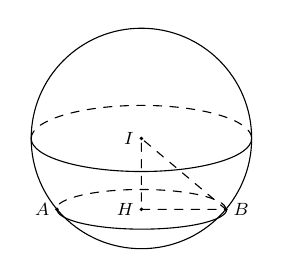
\begin{tikzpicture}[scale=0.7, font=\footnotesize,line join=round, line cap=round, >=stealth]
				\def\r{2}
				\def\a{1}
				\def\b{0.6}
				\pgfmathsetmacro\m{sin(40)}
				\pgfmathsetmacro\n{cos(40)}
				\path
				(0,0) coordinate (O)
				(\r*\n,-\r*\m) coordinate (M)
				(-\r*\n,-\r*\m) coordinate (N)
				(0,-\r*\m) coordinate (H)
				(0,\r) coordinate (A')
				(0,-\r) coordinate (A)
				;
				\draw	(O) circle (\r);
				\node at (O) [left] {$I$};
				\node at (M) [right] {$B$};
				\node at (N) [left] {$A$};
				\node at (H) [left] {$H$};
				%\node at (A') [above] {$A'$};
				%\node at (A) [below] {$A$};
				
				\fill (O) circle (1pt); 
				\fill (M) circle (1pt); 
				\fill (N) circle (1pt); 
				\fill (H) circle (1pt); 
				%\fill (A') circle (1pt); 
				%\fill (A) circle (1pt); 
				
				\draw	(180:\r) arc (180:360:{\r} and	{.3*\r});
				\draw[dashed]	(180:\r) arc (180:0:{\r} and	{.3*\r}) (H)--(M)--(O)--(H);
				
				\draw	(N) arc (180:360:{0.77*\r} and	{0.18*\r});
				\draw [dashed]	(M) arc (0:180:{0.77*\r} and	{0.18*\r});
		\end{tikzpicture}}
	}	
\end{ex}	

\begin{ex}%[2H5H3-2] 
	Trong KG $Oxyz$, cho mặt phẳng $\left( P \right)\colon2x-y-2z-1=0$ và điểm $M\left( 1;-2;0 \right)$. Mặt cầu tâm $M$, bán kính bằng $\sqrt{3}$ cắt mặt phẳng $\left( P \right)$ theo giao tuyến là đường tròn có bán kính bằng bao nhiêu? (\textit{Kết quả làm tròn đến hàng phần trăm}).
	\shortans{$1{,}41$}
	\loigiai{
		\immini{	Mặt cầu tâm tâm $M$, bán kính bằng $R=\sqrt{3}$ cắt phẳng $\left( P \right)$ theo giao tuyến là đường tròn tâm $H$, bán kính $r$ suy ra $r=\sqrt{R^2-MH^2}$.\\
			Với $MH=\mathrm{d}\left( M,\left( P \right) \right)=\dfrac{\left| 2\cdot1-\left( -2 \right)-2\cdot0-1 \right|}{\sqrt{2^2+1^2+2^2}}=1$.\\
			Suy ra $r=\sqrt{{\left( \sqrt{3} \right)^2}-1^2}=\sqrt{2}\approx1{,}41$.}{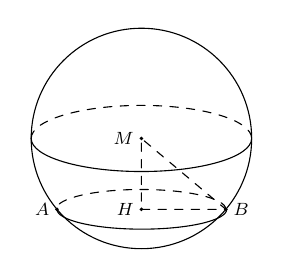
\begin{tikzpicture}[scale=0.7, font=\footnotesize,line join=round, line cap=round, >=stealth]
				\def\r{2}
				\def\a{1}
				\def\b{0.6}
				\pgfmathsetmacro\m{sin(40)}
				\pgfmathsetmacro\n{cos(40)}
				\path
				(0,0) coordinate (O)
				(\r*\n,-\r*\m) coordinate (M)
				(-\r*\n,-\r*\m) coordinate (N)
				(0,-\r*\m) coordinate (H)
				(0,\r) coordinate (A')
				(0,-\r) coordinate (A)
				;
				\draw	(O) circle (\r);
				\node at (O) [left] {$M$};
				\node at (M) [right] {$B$};
				\node at (N) [left] {$A$};
				\node at (H) [left] {$H$};
				%\node at (A') [above] {$A'$};
				%\node at (A) [below] {$A$};
				
				\fill (O) circle (1pt); 
				\fill (M) circle (1pt); 
				\fill (N) circle (1pt); 
				\fill (H) circle (1pt); 
				%\fill (A') circle (1pt); 
				%\fill (A) circle (1pt); 
				
				\draw	(180:\r) arc (180:360:{\r} and	{.3*\r});
				\draw[dashed]	(180:\r) arc (180:0:{\r} and	{.3*\r}) (H)--(M)--(O)--(H);
				
				\draw	(N) arc (180:360:{0.77*\r} and	{0.18*\r});
				\draw [dashed]	(M) arc (0:180:{0.77*\r} and	{0.18*\r});
		\end{tikzpicture}}
	}
\end{ex}

\begin{ex}%[2H5H3-2] 
	Trong không gian với hệ trục tọa độ $Oxyz$, cho mặt phẳng $(P)\colon2x+2y+z-m^2-3m=0$ và mặt cầu $(S)\colon\left( x-1 \right)^2+\left( y+1 \right)^2+\left( z-1 \right)^2=9$. Gọi $T$ là tập hợp tất cả các giá trị của $m$ để $(P)$ tiếp xúc với $(S)$. Tính tổng các phần tử của $T$.
	\shortans{$-3$}
	\loigiai{
		Ta có $(S)\colon\left\{ \begin{aligned}
			& I\left( 1;-1;1 \right) \\
			& R=3 \\
		\end{aligned} \right.$.\\
		$(P)$ tiếp xúc với $(S)$ khi và chỉ khi
		\begin{eqnarray*}
			& & d\left( I;\left( P \right) \right)=R\\
			&\Leftrightarrow & \dfrac{\left| 1-m^2-3m \right|}{3}=3\\
			&\Leftrightarrow & \left[ \begin{aligned}
				& {m^2}+3m-10=0 \\
				& {m^2}+3m+8=0 \\
			\end{aligned} \right.\\
			&\Leftrightarrow & \left[ \begin{aligned}
				& m=2 \\
				& m=-5 \\
			\end{aligned} \right.\\
		\end{eqnarray*}
		Vậy tổng các phần tử của $T$ là $-3$.
	}
\end{ex}

\begin{ex}%[2H5H3-2] 
	Trong không gian $\text{O}xyz$, cho mặt cầu $\left( S \right) \colon {{\left( x-2 \right)}^2}+{{\left( y-4 \right)}^2}+{{\left( z-1 \right)}^2}=4$ và mặt phẳng $\left( P \right): x+my+z-3m-1=0$. Gọi $T$ là tập hợp tất cả các giá trị của $m$ để mặt phẳng $\left( P \right)$ cắt mặt cầu $\left( S \right)$ theo giao tuyến là đường tròn có đường kính bằng $2$. Tính tổng các phần tử của $T$.
	\shortans{$1$}
	\loigiai{
		\immini{	Mặt cầu  $\left(S\right)\colon{{\left( x-2 \right)}^2}+{{\left( y-4 \right)}^2}+{{\left( z-1 \right)}^2}=4$ có tâm $I\left( 2;4;1 \right)$, bán kính $R=2$.\\
			Ta có $\mathrm{d}\left( I,\left( P \right) \right)=\dfrac{\left| 2+4m+1-3m-1 \right|}{\sqrt{1+m^2+1}}$ $=\dfrac{\left| m+2 \right|}{\sqrt{m^2+2}}$\\
			Mặt phẳng $\left( P \right)$ cắt mặt cầu $\left( S \right)$ theo giao tuyến là đường tròn có đường kính bằng $2$ nên bán kính đường tròn giao tuyến là $r=1$.}{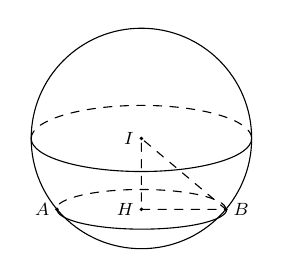
\begin{tikzpicture}[scale=0.7, font=\footnotesize,line join=round, line cap=round, >=stealth]
				\def\r{2}
				\def\a{1}
				\def\b{0.6}
				\pgfmathsetmacro\m{sin(40)}
				\pgfmathsetmacro\n{cos(40)}
				\path
				(0,0) coordinate (O)
				(\r*\n,-\r*\m) coordinate (M)
				(-\r*\n,-\r*\m) coordinate (N)
				(0,-\r*\m) coordinate (H)
				(0,\r) coordinate (A')
				(0,-\r) coordinate (A)
				;
				\draw	(O) circle (\r);
				\node at (O) [left] {$I$};
				\node at (M) [right] {$B$};
				\node at (N) [left] {$A$};
				\node at (H) [left] {$H$};
				%\node at (A') [above] {$A'$};
				%\node at (A) [below] {$A$};
				
				\fill (O) circle (1pt); 
				\fill (M) circle (1pt); 
				\fill (N) circle (1pt); 
				\fill (H) circle (1pt); 
				%\fill (A') circle (1pt); 
				%\fill (A) circle (1pt); 
				
				\draw	(180:\r) arc (180:360:{\r} and	{.3*\r});
				\draw[dashed]	(180:\r) arc (180:0:{\r} and	{.3*\r}) (H)--(M)--(O)--(H);
				
				\draw	(N) arc (180:360:{0.77*\r} and	{0.18*\r});
				\draw [dashed]	(M) arc (0:180:{0.77*\r} and	{0.18*\r});
		\end{tikzpicture}}
		
		Ta có 
		\begin{eqnarray*}
			& & R^2=d^2\left( I,\left( P \right) \right)+r^2\\
			&\Leftrightarrow & 4=\dfrac{{{\left( m+2 \right)}^2}}{m^2+2}+1\\
			&\Leftrightarrow & {m^2}+4m+4=3\left( {m^2}+2 \right)\\
			&\Leftrightarrow & 2m^2-4m+2=0\Leftrightarrow m=1.
		\end{eqnarray*}
	}
\end{ex}

\begin{ex}%[2H5H3-2] 
	Trong không gian với hệ trục toạ độ $Oxyz$, cho mặt cầu có phương trình $\left( S \right)\colon x^2+y^2+z^2+2x-4y-6z+m-3=0$. Gọi $T$ là tập hợp tất cả các giá trị của $m$ để mặt phẳng $\left( \beta \right)\colon2x-y+2z-8=0$ cắt $\left( S \right)$ theo một đường tròn có chu vi bằng $8\pi$. Tính tổng các phần tử của $T$.
	\shortans{$-1$}
	\loigiai{
		Ta có $\left( S \right)\colon x^2+y^2+z^2+2x-4y-6z+m-3=0\Leftrightarrow {{\left( x+1 \right)}^2}+{{\left( y-2 \right)}^2}+{{\left( z-3 \right)}^2}=17-m$.\\
		$\left( S \right)$ là phương trình của mặt cầu thì $17-m>0\Leftrightarrow m<17$.\\
		Khi đó $I\left( -1;2;3 \right);\ R=\sqrt{17-m}$ lần lượt là tâm và bán kính của $\left( S \right)$.\\
		Để mặt phẳng $\left( \beta \right)\colon2x-y+2z-8=0$ cắt $\left( S \right)$ theo thiết diện là một đường tròn có chu vi bằng $8\pi$ thì đường tròn đó có bán kính $r=4$.\\
		Ta có $R^2=d^2\left( I,\left( \beta \right) \right)+r^2\Leftrightarrow 17-m=16+2\Leftrightarrow m=-1$ (TMĐK).}
\end{ex}

\begin{ex}%[2H5H3-2] 
	Trong KG $Oxyz$ cho hai mặt phẳng $\left( P \right)\colon2x-y+z-2=0\,$ và $\left( Q \right)\colon2x-y+z+1=0$. Hỏi có bao nhiêu mặt cầu đi qua $A\left( 1;-2;1 \right)$ và tiếp xúc với hai mặt phẳng $\left( P \right)$, $\left( Q \right)$?
	\shortans{$0$}
	\loigiai{
		Ta có $\left(P\right)\parallel \left(Q\right)$, $M\left( 0;0;2 \right)\in \left( P \right)\Rightarrow \mathrm{d}\left( \left( P \right),\left( Q \right) \right)=\mathrm{d}\left( M,\left( Q \right) \right)=\dfrac{\sqrt{6}}{2}$\\
		$\mathrm{d}\left( A,\left( P \right) \right)=\dfrac{\sqrt{6}}{2}$; $\mathrm{d}\left( A,\left( Q \right) \right)=\sqrt{6}\Rightarrow \mathrm{d}\left( A,\left( Q \right) \right)=\mathrm{d}\left( A,\left( P \right) \right)+\mathrm{d}\left( \left( Q \right),\left( P \right) \right)$.\\
		Vậy không có mặt cầu thỏa yêu cầu bài toán.
	}
\end{ex}

\begin{ex}%[2H5H3-2]% Cau 6
	Trong KG $Oxyz$, cho mặt cầu $\left( S \right)\colon\left( x-1 \right)^2+\left( y-1 \right)^2+z^2=4$ và một điểm $M\left( 2;\,3;\,1 \right)$. Từ $M$ kẻ được vô số các tiếp tuyến tới $\left( S \right)$, biết tập hợp các tiếp điểm là đường tròn $\left( C \right)$. Tính bán kính $r$ của đường tròn $\left( C \right)$. (\textit{Kết quả làm tròn tới hàng phần trăm}).
	\shortans{$1{,}15$}
	\loigiai{
		\immini{	Mặt cầu $\left( S \right)$ có tâm $I\left( 1;1;0 \right)$ và bán kính $R=2$.\\
			Ta có $\overrightarrow{IM}=\left( 1;2;1 \right)$ và $IM=\sqrt{6}$.\\
			Gọi $H$ là một tiếp điểm tùy ý khi kẻ tiếp tuyến từ $M$ đến mặt cầu, khi đó $MH=\sqrt{IM^2-R^2}=\sqrt{2}$. Gọi $O$ là tâm của đường tròn $\left( C \right)$ khi đó $IM\bot HO$ và $HO=r$.\\
			Ta có $HI\cdot HM=HO\cdot IM\Rightarrow r=\dfrac{HI\cdot HM}{IM}=\dfrac{2\sqrt{2}}{\sqrt{6}}=\dfrac{2\sqrt{3}}{3}$.}{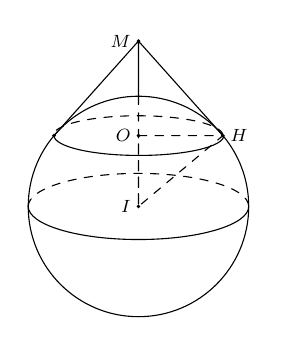
\begin{tikzpicture}[scale=0.7, font=\footnotesize,line join=round, line cap=round, >=stealth]
				\def\r{2}
				\def\a{1}
				\def\b{0.6}
				\pgfmathsetmacro\m{sin(40)}
				\pgfmathsetmacro\n{cos(40)}
				\path
				(0,0) coordinate (O)
				(0,3) coordinate (T)
				(\r*\n,\r*\m) coordinate (M)
				(-\r*\n,\r*\m) coordinate (N)
				(0,\r*\m) coordinate (H)
				(0,\r) coordinate (A')
				(0,-\r) coordinate (A)
				;
				\draw	(O) circle (\r);
				\node at (O) [left] {$I$};
				\node at (M) [right] {$H$};
				%\node at (N) [left] {$A$};
				\node at (H) [left] {$O$};
				\node at (T) [left] {$M$};
				%\node at (A') [above] {$A'$};
				%\node at (A) [below] {$A$};
				
				\fill (O) circle (1pt); 
				\fill (M) circle (1pt); 
				\fill (N) circle (1pt); 
				\fill (H) circle (1pt); 
				\fill (T) circle (1pt); 
				%\fill (A') circle (1pt); 
				%\fill (A) circle (1pt); 
				
				\draw	(180:\r) arc (180:360:{\r} and	{.3*\r}) (T)--(A') (T)--(M) (T)--(N);
				\draw[dashed]	(180:\r) arc (180:0:{\r} and	{.3*\r}) (H)--(M)--(O)--(H) (A')--(O);
				
				\draw	(N) arc (180:360:{0.77*\r} and	{0.18*\r});
				\draw [dashed]	(M) arc (0:180:{0.77*\r} and	{0.18*\r});
		\end{tikzpicture}}
	}
\end{ex}

\begin{ex}%[2H5H3-2] 
	Trong KG $Oxyz$, xét các điểm $A\left( 0;0;1 \right)$, $B\left( m;0;0 \right)$, $C\left( 0;n;0 \right)$, $D\left( 1;1;1 \right)$ với $m>0$; $n>0$ và $m+n=1$. Biết rằng khi $m$, $n$ thay đổi, tồn tại một mặt cầu cố định tiếp xúc với mặt phẳng $\left( ABC \right)$ và đi qua $D$. Tính bán kính $R$ của mặt cầu đó.
	\shortans{$1$}
	\loigiai{		
		Gọi $I\left( 1;1;0 \right)$ là hình chiếu vuông góc của $D$ lên mặt phẳng $(Oxy)$.\\
		Ta có phương trình theo đoạn chắn của mặt phẳng $(ABC)$ là $\dfrac{x}{m}+\dfrac{y}{n}+z=1$.\\
		Suy ra phương trình tổng quát của $(ABC)$ là $nx+my+mnz-mn=0$.\\
		Mặt khác $\mathrm{d}\left( I;\left( ABC \right) \right)=\dfrac{\left| 1-mn \right|}{\sqrt{m^2+n^2+m^2{n^2}}}=1$ (vì $m+n=1$)\\ và $ID=1=d(\left( I, \left( ABC \right) \right).$\\
		Nên tồn tại mặt cầu tâm $I$ (là hình chiếu vuông góc của $D$ lên mặt phẳng $Oxy$) tiếp xúc với $(ABC)$ và đi qua $D$. Khi đó $R=1$.}
\end{ex}
\Closesolutionfile{ans}
\indapan{6}{ans/ans-2C5B3CD3-D1-KQ}
\begin{dang}
	{LẬP PHƯƠNG TRÌNH MẶT CẦU LIÊN QUAN ĐẾN MẶT PHẲNG}
\end{dang}
\TN
\Opensolutionfile{ans}[ans/ans-2C5B3CD3-D2]
\begin{ex}%[2H5H3-2] 
	Trong KG $Oxyz$, viết phương trình mặt cầu có tâm $I\left( 2;1;-4 \right)$ và tiếp xúc với mặt phẳng $\left( \alpha \right)\colon x-2y+2z-7=0$.
	\choice
	{$x^2+y^2+z^2+4x+2y-8z-4=0$}
	{$x^2+y^2+z^2+4x-2y+8z-4=0$}
	{\True $x^2+y^2+z^2-4x-2y+8z-4=0$}
	{$x^2+y^2+z^2-4x-2y-8z-4=0$}
	\loigiai{
		Mặt cầu cần tìm có bán kính $R=\mathrm{d}\left( I,\left( \alpha \right) \right)=\dfrac{\left| 2-2\cdot1+2\cdot\left( -4 \right)-7 \right|}{\sqrt{1^2+{\left( -2 \right)^2}+2^2}}=5$.\\
		Phương trình mặt cầu cần tìm là ${{\left( x-2 \right)}^2}+{{\left( y-1 \right)}^2}+{{\left( z+4 \right)}^2}=25$\\
		$\Leftrightarrow {x^2}+y^2+z^2-4x-2y+8z-4=0$.}
\end{ex}

\begin{ex}%[2H5H3-2] 
	Trong KG $Oxyz$, cho mặt cầu $\left( S \right)$ có tâm $I\left( 3;2;-1 \right)$ và đi qua điểm $A\left( 2;1;2 \right)$. Mặt phẳng nào dưới đây tiếp xúc với $\left( S \right)$ tại $A$?
	\choice
	{$x+y+3z-9=0$}
	{\True $x+y-3z+3=0$}
	{$x+y-3z-8=0$}
	{$x-y-3z+3=0$}
	\loigiai{
		Gọi $\left( P \right)$ là mặt phẳng cần tìm. Khi đó, $\left( P \right)$ tiếp xúc với $\left( S \right)$ tại $A$ khi chỉ khi $\left( P \right)$ đi qua $A\left( 2;1;2 \right)$ và nhận vectơ $\overrightarrow{IA}=\left( -1;-1;3 \right)$ làm vectơ pháp tuyến. Phương trình mặt phẳng $\left( P \right)$ là $-x-y+3z-3=0\Leftrightarrow x+y-3z+3=0$.}
\end{ex}

\begin{ex}%[2H5H3-2] 
	Trong KG $Oxyz$, cho mặt phẳng $\left( P \right)\colon x-2y+2z-2=0$ và điểm $I\left( -1;\,2;\,-1 \right)$. Viết phương trình mặt cầu $\left( S \right)$ có tâm $I$ và cắt mặt phẳng $\left( P \right)$ theo giao tuyến là đường tròn có bán kính bằng $5$.
	\choice
	{$\left( S \right)\colon\left( x+1 \right)^2+\left( y-2 \right)^2+\left( z+1 \right)^2=25$}
	{$\left( S \right)\colon\left( x+1 \right)^2+\left( y-2 \right)^2+\left( z+1 \right)^2=16$}
	{$\left( S \right)\colon\left( x-1 \right)^2+\left( y+2 \right)^2+\left( z-1 \right)^2=34$}
	{\True $\left( S \right)\colon\left( x+1 \right)^2+\left( y-2 \right)^2+\left( z+1 \right)^2=34$}
	\loigiai{
		Gọi $h$ là khoảng cách từ tâm $I$ đến mặt phẳng $\left( P \right)$ ta có:\\
		$h=\mathrm{d}\left( I;\left( P \right) \right)=\dfrac{\left| -1-4-2-2 \right|}{\sqrt{1^2+{{\left( -2 \right)}^2}+2^2}}=3$.\\
		Bán kính mặt cầu $\left( S \right)$ là $R=\sqrt{r^2+h^2}=\sqrt{5^2+3^2}=\sqrt{34}$.\\
		Phương trình mặt cầu $\left( S \right)$ là $\left( x+1 \right)^2+\left( y-2 \right)^2+\left( z+1 \right)^2=34$.}
\end{ex}

\begin{ex}%[2H5H3-3] 
	Trong KG $Oxyz$, mặt cầu $\left( S \right)$ có tâm $I\left( -1;\,2;\,1 \right)$ và tiếp xúc với mặt phẳng $\left( P \right)\colon x-2y-2z-2=0$ có phương trình là
	\choice
	{$\left( x+1 \right)^2+\left( y-2 \right)^2+\left( z-1 \right)^2=3$}
	{$\left( x-1 \right)^2+\left( y+2 \right)^2+\left( z+1 \right)^2=9$}
	{\True $\left( x+1 \right)^2+\left( y-2 \right)^2+\left( z-1 \right)^2=9$}
	{$\left( x+1 \right)^2+\left( y-2 \right)^2+\left( z+1 \right)^2=3$}
	\loigiai{
		Vì mặt cầu tâm $I\left( -1;\,2;\,1 \right)$ tiếp xúc với mặt phẳng $\left( P \right)\colon x-2y-2z-2=0$ nên bán kính\\
		$R=\mathrm{d}\left( I,\,\left( P \right) \right)=\dfrac{\left| -1-2\cdot2-2\cdot1-2 \right|}{\sqrt{1^2+\left( -2 \right)^2+\left( -2 \right)^2}}=3$ $\Rightarrow \left( S \right)\colon\left( x+1 \right)^2+\left( y-2 \right)^2+\left( z-1 \right)^2=9$.}
\end{ex}

\begin{ex}%[2H5H3-3] 
	Trong KG $Oxyz$, cho mặt cầu $\left( S \right)$ có tâm $I\left( 1;2;1 \right)$ và cắt mặt phẳng $\left( P \right)\colon2x-y+2z+7=0$ theo một đường tròn có đường kính bằng $8$. Phương trình mặt cầu $\left( S \right)$ là
	\choice
	{$\left( x-1 \right)^2+\left( y-2 \right)^2+\left( z-1 \right)^2=81$}
	{${{\left( x-1 \right)}^2}+{{\left( y-2 \right)}^2}+{{\left( z-1 \right)}^2}=5$}
	{${{\left( x+1 \right)}^2}+{{\left( y+2 \right)}^2}+{{\left( z+1 \right)}^2}=9$}
	{\True ${{\left( x-1 \right)}^2}+{{\left( y-2 \right)}^2}+{{\left( z-1 \right)}^2}=25$}
	\loigiai{
		
		Khoảng cách từ tâm $I$ đến mặt phẳng $\left( P \right)$ là\\
		$d=\mathrm{d}\left( I,\left( P \right) \right)=\dfrac{\left| 2\cdot1-2+2\cdot1+7 \right|}{\sqrt{2^2+{{\left( -1 \right)}^2}+2^2}}=3$.\\
		Đường tròn giao tuyến có đường kính bằng $8$ nên bán kính đường tròn là $r=4$.\\
		Bán kính của mặt cầu $\left( S \right)$là $R=\sqrt{d^2+r^2}=\sqrt{3^2+4^2}=5$.\\
		Vậy phương trình mặt cầu $\left( S \right)$ là ${{\left( x-1 \right)}^2}+{{\left( y-2 \right)}^2}+{{\left( z-1 \right)}^2}=25$.}
\end{ex}

\begin{ex}%[2H5H3-2] 
	Trong không gian với hệ trục toạ độ $Oxyz$, phương trình nào dưới đây là phương trình của mặt cầu có tâm $I\left( 3;1;0 \right)$ và tiếp xúc với mặt phẳng $\left( P \right): 2x + 2y - z + 1=0$?
	\choice
	{${{\left( x+3 \right)}^2}+{{\left( y+1 \right)}^2}+z^2=3$}
	{${{\left( x+3 \right)}^2}+{{\left( y+1 \right)}^2}+z^2=9$}
	{${{\left( x-3 \right)}^2}+{{\left( y-1 \right)}^2}+z^2=3$}
	{\True ${{\left( x-3 \right)}^2}+{{\left( y-1 \right)}^2}+z^2=9$}
	\loigiai{
		Gọi $\left( S \right)$ là mặt cầu có tâm $I$và tiếp xúc với $\left( P \right)$ có $R$ là bán kính.\\
		Khi đó ta có $\mathrm{d}\left( I,\left( P \right) \right)=R\Rightarrow R=\dfrac{\left| 2\cdot3+2\cdot1-0+1 \right|}{\sqrt{2^2+2^2+{{\left( -1 \right)}^2}}}\Leftrightarrow R=3$.\\
		Vậy phương trình của $\left( S \right)$ là ${{\left( x-3 \right)}^2}+{{\left( y-1 \right)}^2}+z^2=9$.}
\end{ex}

\begin{ex}%[2H5H3-2] 
	Trong KG $Oxyz$, cho mặt cầu $\left( S \right)$ có tâm $I\left( 2;1;1 \right)$ và mặt phẳng $\left( P \right)\colon2x+y+2z+2=0$. Biết mặt phẳng $\left( P \right)$ cắt mặt cầu $\left( S \right)$ theo giao tuyến là một đường tròn có bán kính bằng $1$. Viết phương trình của mặt cầu $\left( S \right)$.
	\choice
	{$\left( S \right)\colon\left( x+2 \right)^2+\left( y+1 \right)^2+\left( z+1 \right)^2=8$}
	{$\left( S \right)\colon\left( x+2 \right)^2+\left( y+1 \right)^2+\left( z+1 \right)^2=10$}
	{$\left( S \right)\colon\left( x-2 \right)^2+\left( y-1 \right)^2+\left( z-1 \right)^2=8$}
	{\True $\left( S \right)\colon\left( x-2 \right)^2+\left( y-1 \right)^2+\left( z-1 \right)^2=10$}
	\loigiai{
		Gọi $R$, $r$ lần lượt là bán kính của mặt cầu $\left( S \right)$ và đường tròn giao tuyến\\
		Ta có ${R^2=r^2+{{\left( \mathrm{d}\left( I,\left( P \right) \right) \right)}^2}=1+{{\left( \dfrac{\left| 2\cdot2+1\cdot1+2\cdot1+2 \right|}{\sqrt{2^2+1+2^2}} \right)}^2}=10}$.\\
		Mặt cầu $\left( S \right)$ tâm $I\left( 2;1;1 \right)$ bán kính $R=\sqrt{10}$ là ${{\left( x-2 \right)}^2}+{{\left( y-1 \right)}^2}+{{\left( z-1 \right)}^2}=10$}
\end{ex}

\begin{ex}%[2H5H3-2] 
	Trong không gian với hệ trục tọa độ $Oxyz$, phương trình nào dưới đây là phương trình mặt cầu đi qua ba điểm $M\left( 2;3;3 \right)$, $N\left( 2;-1;-1 \right)$, $P\left( -2;-1;3 \right)$ và có tâm thuộc mặt phẳng $\left( \alpha \right)\colon2x+3y-z+2=0$?
	\choice
	{$x^2+y^2+z^2+4x-2y+6z+2=0$}
	{$x^2+y^2+z^2-2x+2y-2z-2=0$}
	{$x^2+y^2+z^2-2x+2y-2z-10=0$}
	{\True $x^2+y^2+z^2-4x+2y-6z-2=0$}
	\loigiai{
		Giả sử phương trình mặt cầu $\left( S \right)$ có dạng $x^2+y^2+z^2-2ax-2by-2cz+d=0$.\\
		Điều kiện: $a^2+b^2+c^2-d>0$ \hfill(*) \\
		Vì mặt cầu $\left( S \right)$ đi qua 3 điểm $M\left( 2;3;3 \right)$, $N\left( 2;-1;-1 \right)$, $P\left( -2;-1;3 \right)$ và có tâm $I$ thuộc $mp\left( P \right)$ nên ta có hệ phương trình\\ $\left\{ \begin{aligned}
			& 4a+6b+6c-d=22 \\
			& 4a-2b-2c-d=6 \\
			& 4a+2b-6c+d=-14 \\
			& 2a+3b-c=-2 \\
		\end{aligned} \right.\Leftrightarrow \left\{ \begin{aligned}
			& a=2 \\
			& b=-1 \\
			& c=3 \\
			& d=-2 \\
		\end{aligned} \right.\,\,(\text{thỏa mãn}\left( * \right))$\\
		Vậy phương trình mặt cầu là $x^2+y^2+z^2-4x+2y-6z-2=0.$}
\end{ex}

\begin{ex}%[2H5H3-2] 
	Trong KG $Oxyz$, cho điểm $I(-3;0;1)$. Mặt cầu $(S)$ có tâm $I$ và cắt mặt phẳng $(P)\colon x-2y-2z-1=0$ theo một thiết diện là một hình tròn. Diện tích của hình tròn này bằng $\pi$. Phương trình mặt cầu $(S)$ là
	\choice
	{$(x+3)^2+y^2+(z-1)^2=4$}
	{$(x+3)^2+y^2+(z-1)^2=25$}
	{\True $(x+3)^2+y^2+(z-1)^2=5$}
	{$(x+3)^2+y^2+(z-1)^2=2$}
	\loigiai{
		Gọi $S$, $r$ lần lượt là diện tích hình tròn và bán kính hình tròn.\\
		Ta có $S=\pi r^2=\pi \Rightarrow r=1$.\\
		$\mathrm{d}\left( I, \left( P \right) \right)=\dfrac{\left| -3-2\cdot0-2\cdot1-1 \right|}{\sqrt{1+4+4}}=2$.\\
		$(S)$ có tâm $I(-3;0;1)$ và bán kính $R=\sqrt{\left(\mathrm{d}\left( I,\left( P \right)\right) \right)^2+r^2}=\sqrt{2^2+1^2}=\sqrt{5}$.\\
		Phương trình mặt cầu $(S)$ là $(x+3)^2+y^2+(z-1)^2=5$.}
\end{ex}

\begin{ex}%[2H5H3-2] 
	Trong KG $Oxyz$, cho mặt phẳng $\left( P \right)\colon x-2y+2z-2=0$ và điểm $I\left( -1\,;\,\,2\,;\,\,-1 \right)$. Viết phương trình mặt cầu $\left( S \right)$ có tâm $I$ và cắt mặt phẳng $\left( P \right)$ theo giao tuyến là đường tròn có bán kính bằng $5$.
	\choice
	{$\left( S \right)\colon\left( x+1 \right)^2+\left( y-2 \right)^2+\left( z+1 \right)^2=25$}
	{$\left( S \right)\colon\left( x+1 \right)^2+\left( y-2 \right)^2+\left( z+1 \right)^2=16$}
	{$\left( S \right)\colon\left( x-1 \right)^2+\left( y+2 \right)^2+\left( z-1 \right)^2=34$}
	{\True $\left( S \right)\colon\left( x+1 \right)^2+\left( y-2 \right)^2+\left( z+1 \right)^2=34$}
	\loigiai{
		Gọi $M$ là điểm nằm trên đường tròn giao tuyến của $\left( S \right)$ và $\left( P \right)$. Ta có $IM=R$. Áp dụng công thức tính bán kính mặt cầu trong trường hợp mặt cầu $\left( S \right)$ giao với mặt phẳng $\left( P \right)$ theo giao tuyến là đường tròn có bán kính $r$ là\\
		$IM^2=R^2=d^2\left( I\,,\,\left( P \right) \right)+r^2$ \hfill(*)\\
		Ta có ${\mathrm{d}\left( I,\left( P \right) \right)}=\dfrac{\left| -1-2\cdot2+2\cdot\left( -1 \right)-2 \right|}{\sqrt{1^2+{{\left( -2 \right)}^2}+2^2}}=3=IH$.\\
		Từ $\left( * \right)\Rightarrow {R^2}=3^2+5^2=34$.\\
		Vậy phương trình mặt cầu $\left( S \right)$ thỏa mãn yêu cầu đề bài là\\ ${{\left( x+1 \right)}^2}+{{\left( y-2 \right)}^2}+{{\left( z+1 \right)}^2}=34$.}
\end{ex}
\Closesolutionfile{ans}
\indapan{10}{ans/ans-2C5B3CD3-D2}
\TNSA
\Opensolutionfile{ans}[ans/ans-2C5B3CD3-D2-KQ]
\begin{ex}%[2H5H3-2] 
	Trong KG $Oxyz$, cho điểm $A\left( 1;2;3 \right)$. Tính bán kính của mặt cầu tâm $A$ và tiếp xúc với mặt phẳng $x-2y+2z+3=0$.
	\shortans{$2$}
	\loigiai{
		${{\left( x-1 \right)}^2}+{{\left( y-2 \right)}^2}+{{\left( z-3 \right)}^2}=4$\\
		Mặt cầu tâm $A$ tiếp xúc với mặt phẳng đã cho có bán kính $R=\dfrac{\left| 1-2\cdot2+2\cdot3+3 \right|}{\sqrt{1+4+4}}=2$.}
\end{ex}

\begin{ex}%[2H5H3-2]
	Trong KG $Oxyz$, cho mặt phẳng $(P)\colon x+2 y-2 z+3=0$ và mặt cầu $(S)$ có tâm $I(0 ;-2 ; 1)$. Biết mặt phẳng $(P)$ cắt mặt cầu $(S)$ theo giao tuyến là một đường tròn có diện tích $2 \pi$. Tính bán kính mặt cầu (\textit{kết quả làm tròn đến hàng phần trăm}).
	\shortans{$1{,}73 $}
	\loigiai{
		Gọi $R,$ $r$ lần lượt là bán kính của mặt cầu và đường tròn giao tuyến. Theo giải thiết ta có
		$$
		\pi r^{2}=2 \pi \Leftrightarrow r^{2}=2.
		$$
		Mặt khác $\mathrm{d}(I,(P))=\dfrac{\left| 2\cdot (-2) -2 \cdot 1 +3 \right|}{\sqrt{1^2+ 2^2 +(-2)^2}}=1$ nên $R^{2}=r^{2}+\left[\mathrm d(I,(P))\right]^{2}=3$.\\
		Vậy $R=\sqrt{3}\approx 1{,} 73$.}
\end{ex}

\begin{ex}%[2H5H3-2]
	Trong không gian, cho bốn mặt cầu có bán kính lần lượt là $2$, $3$, $3$, $2$ (đơn vị độ dài) tiếp xúc ngoài với nhau. Mặt cầu nhỏ nhất tiếp xúc ngoài với cả bốn mặt cầu nói trên có bán kính bằng bao nhiêu? (\textit{kết quả làm tròn đến hàng phần trăm}).
	\shortans{$0{,} 55$}
	\loigiai{\immini{
			Gọi $A$, $B$, $C$, $D$ là tâm bốn mặt cầu.\\
			Do các mặt cầu tiếp xúc ngoài với nhau nên không mất tính tổng quát ta giả sử $A B=4$, $A C=B D=A D=B C=5$.\\ Gọi $M, N$ lần lượt là trung điểm của $A B, C D$. Dễ dàng tính được $M N=2 \sqrt{3}$.\\
			Gọi $I$ là tâm mặt cầu nhỏ nhất với bán kính $r$ tiếp xúc với bốn mặt cầu trên. Vì $I A=I B, I C=I D$ nên $I$ nằm trên đoạn $M N$.\\
			Đặt $I N=x$, ta có $I C=\sqrt{3^{2}+x^{2}}=3+r,\break  I A=\sqrt{2^{2}+(2 \sqrt{3}-x)^{2}}=2+r$.
		}{\begin{tikzpicture}[scale=0.8, font=\footnotesize, line join=round, line cap=round, >=stealth]
				%\draw[color=gray,dash pattern=on 1pt off 1pt,xstep=1.0cm,ystep=1.0cm] (-5.2,-5.2) grid (5.2,5.2);
				\coordinate (A) at (0,0);
				\coordinate (D) at ($(A)+ (5,0)$);
				\coordinate (C) at ($(A)+(-60:3)$);
				\coordinate (B) at ($(A)+(60:5)$);
				\coordinate (M) at ($(A)!1/2!(B)$);
				\coordinate (N) at ($(C)!1/2!(D)$);
				\coordinate (I) at ($(M)!1/2!(N)$);
				%\draw pic[draw,angle radius=2mm] {right angle = S--H--K}; 
				%\draw pic[draw,angle radius=2mm] {right angle = H--I--K};
				%\draw pic[draw,angle radius=2mm] {right angle = H--K--D};
				%\coordinate (I) at (intersection of O--N and A--B) {};
				\draw (B)--(A)--(C)--(D)--cycle (C)--(B); 
				\draw[dashed] (A)--(D) (B)--(I)--(A) (C)--(I)--(D) (M)--(I)--(N);
				
				\foreach \p/\r in {A/180,B/90, C/0, D/0,  I/40, M/180, N/0}
				\fill (\p) circle (1.5pt) node[shift={(\r:3mm)}]{$\p$};
			\end{tikzpicture}	
		}
		\noindent
		Từ đó suy ra $\sqrt{3^{2}+x^{2}}-\sqrt{2^{2}+(2 \sqrt{2}-x)^{2}}=1 \Leftrightarrow x=\dfrac{12 \sqrt{3}}{11}$.\\
		Suy ra $r=\sqrt{3^{2}+\left(\dfrac{12 \sqrt{3}}{11}\right)^{2}}-3=\dfrac{6}{11}\approx 0{,} 55$.}
\end{ex}

\begin{ex}%[2H5V3-3]
	Trong KG $Oxyz$, cho mặt cầu $(S)\colon x^{2}+y^{2}+(z-\sqrt{2})^{2}=3$. Có tất cả bao nhiêu điểm $A(a ; b ; c)$, $(a, b, c$ là các số nguyên) thuộc mặt phẳng $(O x y)$ sao cho có ít nhất hai tiếp tuyến của $(S)$ đi qua $A$ và hai tiếp tuyến đó vuông góc với nhau?
	\shortans{$12$}
	\loigiai{
		Mặt cầu $(S)$ có tâm $I\left(0 ; 0 ; \sqrt{2}\right)$ và bán kính $R=\sqrt{3}$.\\
		Do $ A \in(O x y) \Rightarrow A(a ; b ; 0)$.
		\begin{itemize}
			\item Xét trường hợp $A \in(S)$, ta có $a^{2}+b^{2}=1$.\\
			Lúc này các tiếp tuyến của $(S)$ thuộc tiếp diện của $(S)$ tại $A$ nên có vô số các tiếp tuyến vuông góc nhau.
			\\
			Trường hợp này ta có $4$ cặp giá trị của $(a ; b)$ là  $(0;1)$; $(0;-1)$; $(-1;0)$; $(1;0)$.
			\item Xét trường hợp $A$ ở ngoài $(S)$. Khi đó, các tiếp tuyến của $(S)$ đi qua $A$ thuộc mặt nón đỉnh $A$. Nên các tiếp tuyến này chỉ có thể vuông góc với nhau tại $A$.
			\immini{Giả sử $A N ; A M$ là các tiếp tuyến của $(S)$ thỏa mãn $A$, $M$,  $N$,  $I$ đồng phẳng ($N$, $M$ là các tiếp điểm).\\
				Điều kiện để $AM \perp AN$ là góc ở đỉnh của mặt nón lớn hơn hoặc bằng $90^{\circ}$ hay $\widehat{MAN} \ge 90^\circ$.
			}{
				\begin{tikzpicture}[line join=round,scale=.5, line cap=round,thick]
					\pgfmathsetmacro\a{sqrt(13)}
					\def\b{5}
					\coordinate (I) at (2,0);
					\coordinate (A) at (-4,0);
					\coordinate (J) at ($(A)!1/2!(I)$);
					\path[name path=c1] (I) circle (\a);
					\path[name path=c2] (J) let \p1=($(J)-(A)$) in circle ({veclen(\x1,\y1)});
					\draw[dashed, name path=i] (I)--(A);
					\path[name intersections={of=c1 and c2, by={M,N}}];
					\draw[dashed, name path=mn](N)--(M);
					\path[name intersections={of=mn and i, by={K}}];
					%\draw[dashed](-1.5,0) ellipse (0.5 and 1.5);
					%\draw[dashed]  (C) arc (90:-90:{0.5} and {3});
					\draw (M) arc (90:270:{0.5} and {2.9});
					%	\coordinate (B) at (150:{0.5} and {2.9});
					\draw[dashed]  (M) arc (90:-90:{0.5} and {2.9});
					\draw[fill=black] (A) circle(1pt);
					\path (I) circle (\a);
					\begin{scope}
						%\clip (I') circle (\b);
						\draw[dashed] (I) circle (\a);
					\end{scope}
					%\draw (I) circle (\a);
					\begin{scope}
						%	\clip (I') circle (\b);
						\draw[dashed] (I) circle (\a);
					\end{scope}
					\path (3,0) circle (4.25);
					\begin{scope}
						\draw (I) circle (\a);
					\end{scope}
					\draw[dashed] (I)--(M);
					\draw  (M)--(A)--(N);
					\foreach \i/\g in {I/0,M/90,N/-90, A/180}{\draw[fill=black](\i) circle (1pt) ($(\i)+(\g:3mm)$) node[scale=.6]{$\i $};};
			\end{tikzpicture}}
			\noindent
			$$\Leftrightarrow \heva{&I A>R \\ & 90^\circ\ge  \widehat{MAI} \ge 45^\circ} \Leftrightarrow \heva{&IA > \sqrt{3} \\ &\sin \widehat{MAI}= \dfrac{R}{IA}\ge \dfrac{\sqrt{2}}{2}}\Leftrightarrow\heva{&IA > \sqrt{3}\\& IA \le \sqrt{6}}\Leftrightarrow \heva{&a^2 +b^2 > 1 \\& a^2 + b^2 \le 4} $$
			\noindent	 Vì $a, b$ là các số nguyên nên ta có các cặp nghiệm $(a ; b)$ là
			$(0 ; 2)$, $(0 ;-2),$ $(2 ; 0),$ $(-2 ; 0),$ $(1 ; 1)$, $(-1 ;-1)$, $(-1 ; 1)$, $(1 ;-1)$.
		\end{itemize}
		Vậy có $12$ điểm $A$ thỏa mãn yêu cầu.}
\end{ex}

\begin{ex}%[2H5V3-3]
	Trong KG $Oxyz$, cho mặt cầu $(S)\colon x^{2}+y^{2}+(z-1)^{2}=5$. Có tất cả bao nhiêu điểm $A(a, b, c)$ ($a, b, c$ là các số nguyên) thuộc mặt phẳng $(Oxy)$ sao cho có ít nhất hai tiếp tuyến của $(S)$ đi qua $A$ và hai tiếp tuyến đó vuông góc với nhau?
	\shortans{$20$}
	\loigiai{
		Mặt cầu có tâm $I(0 ; 0 ; 1)$, bán kính $R=\sqrt{5}$.
		\\
		Do $ A \in(O x y) \Rightarrow A(a ; b ; 0)$.
		\begin{itemize}
			\item Xét trường hợp $A \in(S)$, ta có $a^{2}+b^{2}=4$.\\
			Lúc này các tiếp tuyến của $(S)$ thuộc tiếp diện của $(S)$ tại $A$ nên có vô số các tiếp tuyến vuông góc nhau.
			\\
			Trường hợp này ta có $4$ cặp giá trị của $(a ; b)$ là  $(0;2)$; $(0;-2)$; $(-2;0)$; $(2;0)$.
			\item Xét trường hợp $A$ ở ngoài $(S)$. Khi đó, các tiếp tuyến của $(S)$ đi qua $A$ thuộc mặt nón đỉnh $A$. Nên các tiếp tuyến này chỉ có thể vuông góc với nhau tại $A$.
			\immini{Giả sử $A N ; A M$ là các tiếp tuyến của $(S)$ thỏa mãn $A, \ M,\  N,  \ I$ đồng phẳng ($N ; M$ là các tiếp điểm).\\
				Điều kiện để $AM \perp AN$ là góc ở đỉnh của mặt nón lớn hơn hoặc bằng $90^{\circ}$ hay $\widehat{MAN} \ge 90^\circ$.
			}{
				\begin{tikzpicture}[line join=round,scale=.5, line cap=round,thick]
					\pgfmathsetmacro\a{sqrt(13)}
					\def\b{5}
					\coordinate (I) at (2,0);
					\coordinate (A) at (-4,0);
					\coordinate (J) at ($(A)!1/2!(I)$);
					\path[name path=c1] (I) circle (\a);
					\path[name path=c2] (J) let \p1=($(J)-(A)$) in circle ({veclen(\x1,\y1)});
					\draw[dashed, name path=i] (I)--(A);
					\path[name intersections={of=c1 and c2, by={M,N}}];
					\draw[dashed, name path=mn](N)--(M);
					\path[name intersections={of=mn and i, by={K}}];
					%\draw[dashed](-1.5,0) ellipse (0.5 and 1.5);
					%\draw[dashed]  (C) arc (90:-90:{0.5} and {3});
					\draw (M) arc (90:270:{0.5} and {2.9});
					%	\coordinate (B) at (150:{0.5} and {2.9});
					\draw[dashed]  (M) arc (90:-90:{0.5} and {2.9});
					\draw[fill=black] (A) circle(1pt);
					\path (I) circle (\a);
					\begin{scope}
						%\clip (I') circle (\b);
						\draw[dashed] (I) circle (\a);
					\end{scope}
					%\draw (I) circle (\a);
					\begin{scope}
						%	\clip (I') circle (\b);
						\draw[dashed] (I) circle (\a);
					\end{scope}
					\path (3,0) circle (4.25);
					\begin{scope}
						\draw (I) circle (\a);
					\end{scope}
					\draw[dashed] (I)--(M);
					\draw  (M)--(A)--(N);
					\foreach \i/\g in {I/0,M/90,N/-90, A/180}{\draw[fill=black](\i) circle (1pt) ($(\i)+(\g:3mm)$) node[scale=.6]{$\i $};};
			\end{tikzpicture}}
			\noindent
			$$\Leftrightarrow \heva{&I A>R \\ & 90^\circ\ge  \widehat{MAI} \ge 45^\circ} \Leftrightarrow \heva{&IA > \sqrt{3} \\ &\sin \widehat{MAI}= \dfrac{R}{IA}\ge \dfrac{\sqrt{2}}{2}}\Leftrightarrow\heva{&IA > \sqrt{5}\\& IA \le \sqrt{10}}\Leftrightarrow \heva{&a^2 +b^2 > 4 \\& a^2 + b^2 \le 9.} $$
			\noindent	 Vì $a, b$ là các số nguyên nên ta có các cặp nghiệm $(a ; b)$ là
			$(0 ; \pm 3)$, $(\pm 1 ;\pm 2),$ $(\pm 2 ; \pm 2),$ $(\pm 2 ; \pm 1),$ $(\pm 3 ; 0)$.
		\end{itemize}
		Vậy có $20$ bộ số thỏa mãn yêu cầu.}
\end{ex}

\begin{ex}%[2H5H3-2]
	Trong KG $Oxyz$, cho điểm $H(1 ; 2 ;-2)$. Mặt phẳng $(\alpha)$ đi qua $H$ và cắt các trục $O x$, $O y$, $O z$ lần lượt tại các điểm $A$, $B$, $C$ sao cho $H$ là trực tâm của tam giác $ABC$. Tính bán kính mặt cầu ngoại tiếp tứ diện $OABC$ (\textit{làm tròn kết quả đến hàng phần trăm}).
	\shortans{$5{,} 51$}
	\loigiai{
		Mặt phẳng $(\alpha)$ cắt các trục $Ox$, $Oy$, $O z$ lần lượt tại các điểm $A(a ; 0 ; 0)$, $B(0 ; b ; 0)$, $C(0 ; 0 ; c)$. Do $H$ là trực tâm tam giác $A B C$ nên $a, b, c \neq 0$ và $OH \perp (ABC)$.\\
		Khi đó $( \alpha) \colon \heva{& \text{qua } H(1;2;-2)\\& \text{một véc-tơ pháp tuyến } \vec{OH}= (1;2;-2)}$ có phương trình $$x + 2x - 2z -9=0.$$
		Suy ra $A(9 ; 0 ; 0)$, $B\left(0 ; \dfrac{9}{2} ; 0\right), C\left(0 ; 0 ;-\dfrac{9}{2}\right)$.
		\\
		Khi đó, giả sử mặt cầu ngoại tiếp tứ diện $O A B C$ có phương trình là:
		$$x^{2}+y^{2}+z^{2}-2 a' x-2 b' y-2 c' z+d=0$$ 
		Với $\left(a'\right)^{2}+\left(b'\right)^{2}+\left(c'\right)^{2}-d>0$.\\
		Vì 4 điểm $O,$ $A$, $B$, $C$ thuộc mặt cầu nên ta có hệ phương trình
		$$
		\heva{& 
			d = 0  \\&
			- 1 8 a ^ { \prime } + d = - 8 1  \\&
			- 9 b ^ { \prime } + d = - \dfrac { 8 1 } { 4 } \\&
			9 c ^ { \prime } + d = - \dfrac { 8 1 } { 4 } } \Leftrightarrow \heva{& 
			d=0 \\&
			a'=\dfrac{9}{2} \\&
			b'=\dfrac{9}{4} \\&
			c'=-\dfrac{9}{4}.}
		$$
		Vậy bán kính  của mặt cầu là $R=\sqrt{\left(\dfrac{9}{2}\right)^{2}+\left(\dfrac{9}{4}\right)^{2}+\left(\dfrac{9}{4}\right)^{2}-0}=\dfrac{9 \sqrt{6}}{4} \approx 5{,}51$.}
\end{ex}

\begin{ex}%[2H5C3-2]
	Trong không gian $O x y z$, mặt cầu $(S)$ đi qua điểm $A(2 ;-2 ; 5)$ và tiếp xúc với ba mặt phẳng $(P)\colon x=1$, $(Q)\colon y=-1$ và $(R)\colon z=1$ có bán kính bằng bao nhiêu?
	\shortans{$3$}
	\loigiai{
		Gọi $I(a ; b ; c)$ và $R$ là tâm và bán kính của $(S)$. Khi đó ta có
		$$R=I A=\mathrm d(I ;(P))= \mathrm d(I ;(Q))=\mathrm d(I ;(R)) \Leftrightarrow R=|a-1|=|b+1|=|c-1| \quad (*).$$ 
		Lại do mặt cầu đi qua $A(2;-2;5)$ nên ta suy ra $a>1$, $b<-1$ và $c>1$.\\
		Do đó $(*) \Leftrightarrow \heva{& a-1= -b-1\\ & a-1 = c-1}\Leftrightarrow \heva{& b= -a\\& c=a.}$\\
		Suy ra $(S) \colon (x-a)^2 + (y+a)^2 + (z-a)^2 = (a-1)^2$.\\
		Mà $A(2;-2;5) \in (S)$ nên $(2-a)^2 + (-2+a)^2 + (5-a)^2 = (a-1)^2\Leftrightarrow a=4$.\\
		Vậy $R= |a-1|=3.$}
\end{ex}

\begin{ex}%[2H5C3-2]
	Trong KG $Oxyz$, xét số thực $m \in(0 ; 1)$ và hai mặt phẳng $(\alpha)\colon 2 x-y+2 z+10=0$ và $(\beta)\colon \dfrac{x}{m}+\dfrac{y}{1-m}+\dfrac{z}{1}=1$. Biết rằng, khi $m$ thay đổi có hai mặt cầu cố định tiếp xúc đồng thời với cả hai mặt phẳng $(\alpha)$, $(\beta)$. Tổng bán kính của hai mặt cầu đó bằng bao nhiêu?
	\shortans{$ 9$}
	\loigiai{
		Gọi $I(a ; b ; c)$ là tâm mặt cầu.\\
		Ta có $(\beta) \colon \dfrac{x}{m}+ \dfrac{y}{1-m}+ z=1 \Leftrightarrow  (1-m)x + m y + (m-m^2) z + m^2 -m=0$.\\
		Theo giả thiết 
		\allowdisplaybreaks
		\begin{eqnarray*}
			& R  =\mathrm d (I, (\beta))&=\dfrac{\left|(1-m)a + mb + (m-m^2) c + m^2 -m \right|}{\sqrt{(1-m)^2 + m^2 +(m-m^2)^2 }}\\
			&&=\dfrac{\left|(1-m)a + mb + (m-m^2) c + m^2 -m \right|}{m^2 -m +1}.
		\end{eqnarray*}
		Do $R$ cố định với mọi $m$ nên tồn tại hằng số $k$ thỏa mãn 
		\allowdisplaybreaks
		\begin{eqnarray*}
			&&(1-m)a + mb + (m-m^2) c + m^2 -m  = k \cdot (m^2 -m +1), \, \forall m \\
			&\Leftrightarrow & (1-c)m^2 + (-a + b +c-1) m + a = km^2 - m k + k, \, \forall m\\
			& \Leftrightarrow & \heva{& 1-c = k \\ & -a+b + c-1= -m \\& a = k}\\
			& \Leftrightarrow & \heva{& a =k \\ & b= k \\& c= 1-k.}
		\end{eqnarray*}
		Suy ra $I (k; k; 1-k)$.\\
		Mặt khác $R = \mathrm d (I, (\alpha))$ nên $$R=\dfrac{\left| 2k - k + 2 (1-k) +10\right|}{\sqrt{2^2 + 1^2 + 2^2}}= \dfrac{\left| -k +12\right|}{3}.$$
		Khi đó $\dfrac{\left|-k +2 \right|}{3} = k \Leftrightarrow \hoac{& k=-6 &&\Rightarrow  R= 6\\& k=3 &&\Rightarrow R=3.}$\\
		Vậy $6+3 =9. $}
\end{ex}

\begin{ex}%[2H5C3-2]
	Trong KG $Oxyz$, cho điểm $A(2 ; 11 ;-5)$ và mặt phẳng $(P)\colon 2 m x+\left(m^{2}+1\right) y+\left(m^{2}-1\right) z-10=0$. Biết rằng khi $m$ thay đổi, tồn tại hai mặt cầu cố định tiếp xúc với mặt phẳng $(P)$ và cùng đi qua $A$. Tổng bán kính của hai mặt cầu đó bằng bao nhiêu? (\textit{kết quả làm tròn đến hàng phần chục}).
	\shortans{$17$}
	\loigiai{
		Gọi $I\left(x_{0} ; y_{0} ; z_{0}\right)$ là tâm của mặt cầu $(S)$ cố định và $R$ là bán kính của mặt cầu $(S)$.
		\\
		Ta có
		\allowdisplaybreaks
		\begin{eqnarray*}
			&R=\mathrm  d(I,(P))& =\dfrac{\left|2 m x_{0}+\left(m^{2}+1\right) y_{0}+\left(m^{2}-1\right) z_{0}-10\right|}{\sqrt{4 m^{2}+\left(m^{2}+1\right)^{2}+\left(m^{2}-1\right)^{2}}}\\
			&&=\dfrac{\left|2 m x_{0}+\left(m^{2}+1\right) y_{0}+\left(m^{2}-1\right) z_{0}-10\right|}{\sqrt{2}\cdot \left(m^{2}+1\right)}
		\end{eqnarray*}
		Do tại hai mặt cầu cố định tiếp xúc với $(P)$ nên tồn tại số thực $k$ thỏa mãn \allowdisplaybreaks
		\begin{eqnarray*}
			&& 2m x_0 + (m^2 +1 ) y_0 + (m^2 -1) z_0 -10 = k  \cdot (m^2 +1) \, \forall m\\
			& \Leftrightarrow & (y_0 + z_0) m^2 + 2x_0 m + y_0 -z_0 -10 = k m^2 + k \, \forall m\\
			& \Leftrightarrow & \heva{& y_0+ z_0 =  k \\ & 2x_0 =0 \\& y_0-z_0-10=  k }\\
			& \Leftrightarrow & \heva{ &x_0=0 \\ & y_0= 5 +k \\
				& z_0 = -5.}
		\end{eqnarray*} 
		Suy ra $I \left( 0; 5 + k ; -5 \right)$ và $R = \dfrac{|k|}{\sqrt{2}}$.\\
		Mặt khác 
		\allowdisplaybreaks
		\begin{eqnarray*}
			&R= IA &\Leftrightarrow \dfrac{|k|}{\sqrt{2}}= \sqrt{2^2 + \left(6-k \right)^2}\\
			&&\Leftrightarrow k^2 = 2 \cdot \left(40 + k^2 - 12 k \right) \\
			& &\Leftrightarrow  k^2 -24k + 80=0\\
			&  &\Leftrightarrow  \hoac{& k=4  &&\Rightarrow R= 2\sqrt{2} \\& k=20 &&\Rightarrow R= 10\sqrt{2}.}
		\end{eqnarray*}
		Vậy tổng hai bán kính của hai mặt cầu là $12 \sqrt{2}\approx 17.$}
\end{ex}

\begin{ex}%[2H5C3-2]
	Trong KG $Oxyz$ cho $A(-3 ; 1 ; 1)$,  $B(1 ;-1 ; 5)$ và mặt phẳng $(P)\colon 2 x-y+2 z+11=0$. Mặt cầu $(S)$ đi qua hai điểm $A$, $B$ và tiếp xúc với $(P)$ tại điểm $C$. Biết $C$ luôn thuộc một đường tròn $(T)$ cố định. Tính bán kính $r$ của đường tròn $(T)$.
	\shortans{$4$}
	\loigiai{\immini{Ta có $\overrightarrow{A B}=(4 ;-2 ; 4)$ và $(P)$ có véc-tơ pháp tuyến \break $\vec{n}=(2 ;-1 ; 2)$. Do $\vec{AB}= 2 \cdot \vec{n}$ nên $AB$ vuông góc với $(P)$.
			\\
			Gọi $M$ là trung điểm $AB$. Do $A$, $B \in (S)$ nên $IM \perp AB$ hay $I$ thuộc mặt phẳng trung trực $(Q)$ của đoạn thẳng $AB$.\\
			Ta có $M(-1; 0; 3)$ và $(Q) \colon 2x - y + 2z -4=0$.}{
			\begin{tikzpicture}[line join=round,scale=.5, line cap=round,thick]
				\coordinate (H) at (0,0);
				\coordinate (C) at (5,0);
				\coordinate (I) at ($(C)+(90:3)$);
				\draw[name path=c1] (I) circle (3);
				\coordinate (A) at ($(I)+(140:3)$);
				\coordinate (B) at ($(I)+(-140:3)$);
				\coordinate (M) at ($(A)!1/2!(B)$);
				\draw  (A)--(B) (M)--(I)--(C);
				\draw (1,0)--(9,0);
				\node[above]  at (9,0){$(P)$}; 
				\draw[dashed] ;
				\foreach \i/\g in {I/90,C/-90, B/180, A/90,M/180}{\draw[fill=black](\i) circle (1pt) ($(\i)+(\g:3mm)$) node[scale=.6]{$\i $};};
		\end{tikzpicture}} \noindent
		Suy ra $R = \mathrm d ((P), (Q))= \dfrac{|11+4|}{\sqrt{2^2 +(-1)^2 + 2^2}}=3$.
		\\
		Do $(S)$ tiếp xúc $(P)$ tại $C$ nên $\mathrm d (I, AB) = \mathrm d (C, AB)\Leftrightarrow \mathrm d (C, AB)= \sqrt{R^2 - \dfrac{AB^2}{4}}= 4$.\\
		Vậy $C$ luôn thuộc một đường tròn $(T)$ cố định có bán kính $r=4$.}
\end{ex}

\begin{ex}%[2H5C3-3]
	Trong KG $Oxyz$, cho các điểm $M(2 ; 1 ; 4)$, $N(5 ; 0 ; 0)$, $P(1 ;-3 ; 1)$. Gọi $I(a ; b ; c)$ là tâm của mặt cầu tiếp xúc với mặt phẳng $(Oyz)$ đồng thời đi qua các điểm $M$, $N$, $P$. Tìm $c$ biết rằng $a+b+c<5$.
	\shortans{$2$}
	\loigiai{
		Phương trình mặt cầu $(S)$ tâm $I(a ; b ; c)$.\\
		Do $(S)$ tiếp xúc với $(Oyz)$ nên $R= |a|$.\\
		Suy ra $(S) \colon (x-a)^2 + (y-b)^2 + (z-c)^2 =a^2$.\\
		Mặt khác, $M$, $N$, $P \in (S)$ nên 
		\allowdisplaybreaks
		\begin{eqnarray*}
			&& \heva{&  (2-a)^2 + (1-b)^2 + (4-c)^2 = a^2\\
				& (5-a)^2 + b^2 + c^2 = a^2 \\
				& (1-a)^2 + (3+b)^2 + (1-c)^2 =a^2}\\
			& \Leftrightarrow & \heva{& b^2 + c^2 -2b - 8c - 4a =-21\\
				& b^2 + c^2 -10a = -25\\
				& b^2 + c^2 + 6b -2c -2a = -11}	\\
			& \Leftrightarrow & \heva{& 6a -2b - 8c = 4\\& 8a + 6b -2c = 14\\ & b^2 + c^2 -10a =-25}\\
			& \Leftrightarrow & \heva{& c=a-1\\&b= 2-a \\& (2-a)^2 + (a-1)^2 -10=-25 }\\
			& \Leftrightarrow & \hoac{& \heva{& a= 3\\&b=-1\\&c=2}\\&\heva{&a=5 \\&b=-3\\&c=4.}}
		\end{eqnarray*}Do $a+b+c <5$ nên $\heva{&a=3\\& b=-1\\&c =2.}$ 
	}
\end{ex}
\Closesolutionfile{ans}
\indapan{6}{ans/ans-2C5B3CD3-D2-KQ}
\begin{dang}
	{LẬP PHƯƠNG TRÌNH MẶT PHẲNG LIÊN QUAN ĐẾN MẶT PHẲNG, MẶT CẦU}
\end{dang}
\Opensolutionfile{ans}[ans/ans-2-C5B3CD3-LC]
\TN
\begin{ex}%[2H5H1-3]
	Trong không gian tọa độ $Oxyz$, cho mặt cầu $(S)$ có đường kính $AB$ với $A(6;2;-5)$, $B(-4;0;7)$. Viết phương trình mặt phẳng $(P)$ tiếp xúc với mặt cầu $(S)$ tại $A$.
	\choice
	{$(P)\colon 5x+y-6z+62=0$}
	{\True $(P)\colon 5x+y-6z-62=0$}
	{$(P)\colon 5x-y-6z-62=0$}
	{$(P)\colon 5x+y+6z+62=0$}
	\loigiai{
		Gọi $I$ là trung điểm của $AB$ $\Rightarrow I(1;1;1)$.\\
		Mặt cầu $(S)$ có đường kính $AB$ nên có tâm là điểm $I$.\\
		Mặt phẳng $(P)$ tiếp xúc với mặt cầu $(S)$ tại $A$ nên mặt phẳng $(P)$ đi qua $A$ và nhận $\overrightarrow{IA}=(5;1;-6)$ là véc-tơ pháp tuyến.\\
		Phương trình mặt phẳng $(P)\colon 5(x-6)+1(y-2)-6(z+5)=0\Leftrightarrow 5x+y-6z-62=0$.
	}
\end{ex}
\begin{ex}%[2H5H1-3]
	Trong KG $Oxyz$, cho mặt phẳng $(Q)$ song song với mặt phẳng $(P)\colon 2x-2y+z+7=0$. Biết mp$(Q)$ cắt mặt cầu $(S)\colon x^2+(y+2)^2+(z-1)^2=25$ theo một đường tròn có bán kính $r=3$. Khi đó mặt phẳng $(Q)$ có phương trình là
	\choice
	{$x-y+2z-7=0$}
	{$2x-2y+z+17=0$}
	{$2x-2y+z+7=0$}
	{\True $2x-2y+z-17=0$}
	\loigiai{
		$(S)$ có tâm $I(0;-2;1)$ và bán kính $R=5$.\\
		Gọi $M$ là hình chiếu vuông góc của $I$ lên $(Q)$.\\
		$(Q)$ cắt mặt cầu $(S)$ theo một đường tròn có bán kính $r=3$.\\
		$\Rightarrow IM=\sqrt{R^2-r^2}=\sqrt{5^2-3^2}=4$.\\
		$(Q)\parallel (P)\colon 2x-2y+z+7=0 \Rightarrow (Q)\colon 2x-2y+z+m=0 \quad (m\ne 7)$.
		\begin{eqnarray*}
			\mathrm{d}(I,(Q))&=&\dfrac{|2\cdot 0-2\cdot (-2)+1\cdot 1 +m|}{\sqrt{2^2+(-2)^2+1^2}}=IM=4.\\
			&\Leftrightarrow& |m+5|=12\Leftrightarrow \hoac{&m=7\\ &m=-17.}
		\end{eqnarray*}
		Vậy phương trình của $(Q)$ là $2x-2y+z-17=0$.
	}
\end{ex}
\begin{ex}%[2H5H1-3]
	Trong KG $Oxyz$ cho mặt cầu $(S)\colon x^2+y^2+z^2+2x-4y-6z+5=0$. Mặt phẳng tiếp xúc với $(S)$ và song song với mặt phẳng $(P)\colon 2x-y+2z-11=0$ có phương trình là
	\choice
	{$2x-y+2z-7=0$}
	{$2x-y+2z+9=0$}
	{\True $2x-y+2z+7=0$}
	{$2x-y+2z-9=0$}
	\loigiai{
		Ta gọi phương trình mặt phẳng song song với mặt phẳng $(P)\colon 2x-y+2z-11=0$ có dạng là $(Q)\colon 2x-y+2z+D=0 \quad (D\ne -11)$.\\
		Mặt cầu $(S)$ có tâm $I(-1;2;3)$, bán kính $R=\sqrt{(-1)^2+2^2+3^2-5}=3$.\\
		Vì mặt phẳng tiếp xúc với $(S)$ nên ta có:
		\begin{eqnarray*}
			\mathrm{d}(I,(Q))=R&\Leftrightarrow& \dfrac{|2\cdot(-1)-2+2\cdot 3+D|}{\sqrt{2^2+(-1)^2+2^2}}=3\\
			&\Leftrightarrow& \dfrac{|2+D|}{3}=3 \Leftrightarrow \hoac{&2+D=9\\ &2+D=-9} \Leftrightarrow \hoac{&D=7\\ &D=-11.}
		\end{eqnarray*}
		Do $D\ne -11\Rightarrow D=7$.\\
		Vậy mặt phẳng cần tìm là $2x-y+2z+7=0$.
	}
\end{ex}
\begin{ex}%[2H5H1-3]
	Trong KG $Oxyz$, mặt phẳng $(P)$ chứa trục $Ox$ và cắt mặt cầu $(S)\colon x^2+y^2+z^2-2x+4y+2z-3=0$ theo giao tuyến là đường tròn có bán kính bằng $3$ có phương trình là
	\choice
	{\True $y-2z=0$}
	{$y+2z=0$}
	{$y+3z=0$}
	{$y-3z=0$}
	\loigiai{
		$(S)\colon x^2+y^2+z^2-2x+4y+2z-3=0$ có tâm $I(1;-2;-1)$ và bán kính $R=3$.\\
		$(P)$ cắt mặt cầu $(S)$ theo giao tuyến là đường tròn có bán kính $r=3=R$.\\
		$\Rightarrow I\in (P)$.\\
		Chọn điểm $M(1;0;0)\in Ox\Rightarrow \overrightarrow{IM}=(0;2;1)$.\\
		$\overrightarrow{n}=\left[\overrightarrow{i},\overrightarrow{IM}\right]=(0;-1;2)$.\\
		$(P)$ qua $O(0;0;0)$ và có VTPT $\overrightarrow{n}=(0;-1;2)\Rightarrow (P)\colon y-2z=0$.
	}
\end{ex}
\begin{ex}%[2H5V1-3]
	Trong KG $Oxyz$, cho mặt cầu $(S)\colon x^2+y^2+z^2+2z-2=0$ và điểm $K(2;2;0)$. Viết phương trình mặt phẳng chứa tất cả các tiếp điểm của các tiếp tuyến vẽ từ $K$ đến mặt cầu $(S)$.
	\choice
	{$2x+2y+z-4=0$}
	{$6x+6y+3z-8=0$}
	{\True $2x+2y+z+2=0$}
	{$6x+6y+3z-3=0$}
	\loigiai{
		$(S)\colon x^2+y^2+(z+1)^2=3 \Rightarrow $ mặt cầu tâm $I(0;0;-1)$, $R=\sqrt{3}$.\\
		Do $\overrightarrow{IK}=(2;2;1)$, $IK=3>R\Rightarrow K$ nằm ngoài mặt cầu. Suy ra từ $K$ vẽ được vô số tiếp tuyến đến mặt cầu và khoảng cách từ $K$ đến các tiếp điểm bằng nhau.\\
		Gọi $E$ là $1$ tiếp điểm $\Rightarrow IE\perp EK\Rightarrow \triangle IKE$ vuông tại $E\Rightarrow KE=\sqrt{IK^2-IE^2}=\sqrt{6} \Rightarrow E$ thuộc mặt cầu tâm $K$ bán kính $R'=\sqrt{6}$.\\
		Tọa độ điểm $E$ thỏa mãn hệ\\ $\heva{&x^2+y^2+z^2+2z-2=0\\ &(x-2)^2+(y-2)^2+z^2=6} \Rightarrow x^2+y^2+z^2+2z-2=(x-2)^2+(y-2)^2+z^2=6$.\\
		$\Leftrightarrow 4x+4y+2z+4=0\Leftrightarrow 2x+2y+z+2=0$.
	}
\end{ex}
\begin{ex}%[2H5V1-3]
	Trong KG $Oxyz$, cho mặt cầu $(S)\colon x^2+y^2+z^2-2x+6y-4z-2=0$ và mặt phẳng $(\alpha)\colon x+4y+z-11=0$. Viết phương trình mặt phẳng $(P)$, biết $(P)$ song song với giá của véc-tơ $\overrightarrow{v}=(1;6;2)$, vuông góc với $(\alpha)$ và tiếp xúc với $(S)$.
	\choice
	{$\hoac{&x-2y+z+3=0\\ &x-2y+z-21=0}$}
	{$\hoac{&3x+y+4z+1=0\\ &3x+y+4z-2=0}$}
	{$\hoac{&4x-3y-z+5=0\\ &4x-3y-z-27=0}$}
	{\True $\hoac{&2x-y+2z+3=0\\ &2x-y+2z-21=0}$}
	\loigiai{
		Mặt cầu $(S)$ có tâm $I(1;-3;2)$ và bán kính $R=4$.\\
		Vì mặt phẳng $(P)$ song song với giá của véc-tơ $\overrightarrow{v}=(1;6;2)$, vuông góc với $(\alpha)$ nên có véc-tơ pháp tuyến $\overrightarrow{n}=\left[\overrightarrow{n}_{(\alpha)},\overrightarrow{v}\right]=(2;-1;2)$.\\
		Mặt phẳng $(P)\colon 2x-y+2z+D=0$.\\
		Vì $(P)$ tiếp xúc với mặt cầu $(S)$ nên ta có:
		\begin{eqnarray*}
			\mathrm{d}(I,(P))=R&\Leftrightarrow& \dfrac{|2\cdot 1 +3+ 2\cdot 2+D|}{\sqrt{2^2+(-1)^2+2^2}}=4\\
			&\Leftrightarrow& |D+9|=12\Leftrightarrow \hoac{&D=-21\\ &D=3.}
		\end{eqnarray*}
		Vậy phương trình mặt phẳng $(P)$ là $\hoac{&2x-y+2z+3=0\\ &2x-y+2z-21=0.}$
	}
\end{ex}
\begin{ex}%[2H5V1-3]
	Trong không gian với hệ trục tọa độ $Oxyz$, cho mặt phẳng $(P)$ có phương trình $x-2y-2z-5=0$ và mặt cầu $(S)$ có phương trình $(x-1)^2+(y+2)^2+(z+3)^2=4$. Tìm phương trình mặt phẳng song song với mặt phẳng $(P)$ đồng thời tiếp xúc với mặt cầu $(S)$.
	\choice
	{$x-2y-2z+1=0$}
	{$-x+2y+2z+5=0$}
	{$x-2y-2z-23=0$}
	{\True $-x+2y+2z+17=0$}
	\loigiai{
		Mặt cầu $(S)$ có tâm $I(1;-2;-3)$ và bán kính $R=2$.\\
		Gọi $(Q)$ là mặt phẳng song song với mặt phẳng $(P)$ đồng thời tiếp xúc với mặt cầu $(S)$.\\
		Phương trình $(Q)$ có dạng: $x-2y-2z+D=0$ \quad $(D\ne -5)$.\\
		$(Q)$ tiếp xúc với $(S)$ khi và chỉ khi
		\begin{eqnarray*}
			\mathrm{d}(I,(Q))=R &\Leftrightarrow& \dfrac{|1-2\cdot (-2)-2\cdot (-3)+D|}{\sqrt{1^2+2^2+2^2}}=2\\
			&\Leftrightarrow& |D+11|=6 \Leftrightarrow \hoac{&D+11=6\\ &D+11=-6}\\
			&\Leftrightarrow& \hoac{&D=-5\\ &D=-17.}
		\end{eqnarray*}
		Đối chiếu điều kiện suy ra $D=-17$.\\
		Vậy phương trình của $(Q)$ là $x-2y-2z-17=0 \Leftrightarrow -x+2y+2z+17=0$.
	}
\end{ex}
\begin{ex}%[2H5V1-3]
	Trong không gian với hệ trục tọa độ $Oxyz$ cho mặt cầu $(S)\colon x^2+y^2+z^2-2x+6y-4z-2=0$, mặt phẳng $(\alpha)\colon x+4y+z-11=0$. Gọi $(P)$ là mặt phẳng vuông góc với $(\alpha)$, $(P)$ song song với giá của véc-tơ $\overrightarrow{v}=(1;6;2)$ và $(P)$ tiếp xúc với $(S)$. Lập phương trình mặt phẳng $(P)$.
	\choice
	{$2x-y+2z-2=0$ và $x-2y+z-21=0$}
	{$x-2y+2z+3=0$ và $x-2y+z-21=0$}
	{\True $2x-y+2z+3=0$ và $2x-y+2z-21=0$}
	{$2x-y+2z+5=0$ và $2x-y+2z-2=0$}
	\loigiai{
		$(S)$ có tâm $I(1;-3;2)$ và bán kính $R=4$. Véc-tơ pháp tuyến của $(\alpha)$ là $\overrightarrow{n}_{\alpha}=(1;4;1)$.\\
		Suy ra VTPT của $(P)$ là $\overrightarrow{n}_P=\left[\overrightarrow{n}_{\alpha},\overrightarrow{v}\right]=(2;-1;2)$.\\
		Do đó $(P)$ có dạng: $2x-y+2z+d=0$.\\
		Mặt khác $(P)$ tiếp xúc với $(S)$ nên $\mathrm{d}(I,(P))=4$.\\
		Hay $\dfrac{|2+3+4+d|}{\sqrt{2^2+(-1)^2+2^2}}=4 \Rightarrow \hoac{&d=-21\\ &d=3.}$
	}
\end{ex}
\begin{ex}%[2H5V1-3]
	Trong KG $Oxyz$, viết phương trình mặt phẳng tiếp xúc với mặt cầu $(x-1)^2+y^2+(z+2)^2=6$ đồng thời song song với hai đường thẳng $d_1\colon \dfrac{x-2}{3}=\dfrac{y-1}{-1}=\dfrac{z}{-1}$, $d_2\colon \dfrac{x}{1}=\dfrac{y+2}{1}=\dfrac{z-2}{-1}$.
	\choice
	{$\hoac{&x-y+2z-3=0\\ &x-y+2z+9=0}$}
	{\True $\hoac{&x+y+2z-3=0\\ &x+y+2z+9=0}$}
	{$x+y+2z+9=0$}
	{$x-y+2z+9=0$}
	\loigiai{
		Đường thẳng $d_1$ có vtcp $\overrightarrow{u}_1(3;-1;-1)$, đường thẳng $d_2$ có vtcp $\overrightarrow{u}_2(1;1;-1)$. Gọi $\overrightarrow{n}$ là vtpt của mặt phẳng $(\alpha)$ cần tìm. Do $(\alpha)$ song song với hai đường thẳng $d_1$, $d_2$ nên $\overrightarrow{n}\perp \overrightarrow{u}_1$ và $\overrightarrow{n}\perp \overrightarrow{u}_2$, từ đó ta chọn $\overrightarrow{n}=\left[\overrightarrow{u}_1,\overrightarrow{u}_2\right]=(2;2;4)$. Suy ra $(\alpha)\colon x+y+2z+c=0$.\\
		Mặt cầu $(S)$ có tâm $I(1;0;-2)$, bán kính $R=\sqrt{6}$.\\
		$(\alpha)$ tiếp xúc với $(S)\Leftrightarrow \mathrm{d}(I,(\alpha))=\sqrt{6} \Leftrightarrow \dfrac{|c-3|}{\sqrt{6}}=\sqrt{6} \Leftrightarrow \hoac{&c-3=6\\ &c-3=-6} \Leftrightarrow \hoac{&c=9\\ &c=-3.}$
	}
\end{ex}
\begin{ex}%[2H5V1-3]
	Trong KG $Oxyz$, cho mặt phẳng $(P)$ chứa đường thẳng $d\colon \dfrac{x-4}{3}=\dfrac{y}{1}=\dfrac{z+4}{-4}$ và tiếp xúc với mặt cầu $(S)\colon (x-3)^2+(y+3)^2+(z-1)^2=9$. Khi đó $(P)$ song song với mặt phẳng nào sau đây?
	\choice
	{$3x-y+2z=0$}
	{$-2x+2y-z+4=0$}
	{$x+y+z=0$}
	{\True Đáp án khác}
	\loigiai{
		Véc-tơ chỉ phương của $d$ là $\overrightarrow{u}=(3;1;-4)$, véc-tơ pháp tuyến của mặt phẳng $(P)$ là $\overrightarrow{n}$.\\
		Mặt cầu $(S)$ có tâm $I(3;-3;1)$ và bán kính $R=3$.\\
		Vì $(P)$ chứa $d$ nên $\overrightarrow{u}\cdot \overrightarrow{n}=0$ và $(P)$ tiếp xúc với $(S)$ nên $\mathrm{d}(I,(P))=3$.\\
		Ta chỉ xét phương trình $\overrightarrow{u}\cdot \overrightarrow{n}=0$. Lấy hai điểm nằm trên đường thẳng $d$ là $M(4;0;-4)$ và $N(1;-1;0)$.\\
		Ta nhận thấy: $M(4;0;-4)$ và $N(1;-1;0)$ không thỏa mãn đáp án $A$, $B$, $C$.
	}
\end{ex}
\begin{ex}%[2H5V1-3]
	Trong KG $Oxyz$, cho mặt cầu $(S)\colon (x+1)^2+(y-1)^2+(z+2)^2=2$ và hai đường thẳng $d\colon \dfrac{x-2}{1}=\dfrac{y}{2}=\dfrac{z-1}{-1}$; $\Delta \colon \dfrac{x}{1}=\dfrac{y}{1}=\dfrac{z-1}{-1}$. Phương trình nào dưới đây là phương trình của một mặt phẳng tiếp xúc với $(S)$, song song với $d$ và $\Delta$?
	\choice
	{$y+z+3=0$}
	{\True $x+z+1=0$}
	{$x+y+1=0$}
	{$x+z-1=0$}
	\loigiai{
		Mặt cầu $(S)$ có tâm $I(-1;1;-2)$; $R=\sqrt{2}$.\\
		Véc-tơ chỉ phương của $d\colon \overrightarrow{u}_d=(1;2;-1)$. Véc-tơ chỉ phương của $\Delta$ là $\overrightarrow{u}_{\Delta}=(1;1;-1)$.\\
		Gọi $(P)$ là mặt phẳng cần viết phương trình.\\
		Ta có $\left[\overrightarrow{u}_d,\overrightarrow{u}_{\Delta}\right]=(-1;0;-1)$ nên chọn một véc-tơ pháp tuyến của $(P)$ là $\overrightarrow{n}=(1;0;1)$.\\
		Mặt phẳng $(P)$ có phương trình tổng quát dạng: $x+z+D=0$.\\
		Do $(P)$ tiếp xúc với $(S)$ nên
		\begin{eqnarray*}
			\mathrm{d}(I,(P))=R &\Leftrightarrow& \dfrac{|-1-2+D|}{\sqrt{2}}=\sqrt{2}\\
			&\Leftrightarrow& |D-3|=2 \Leftrightarrow \hoac{&D=5\\ &D=1.}
		\end{eqnarray*}
		Vậy phương trình của $(P)$ là $x+z+1=0$.
	}
\end{ex}
\begin{ex}%[2H5V1-3]
	Trong KG $Oxyz$, cho mặt cầu $(S)\colon (x-1)^2+(y-2)^2+(z-3)^2=1$, đường thẳng $\Delta \colon \dfrac{x-6}{-3}=\dfrac{y-2}{2}=\dfrac{z-2}{2}$ và điểm $M(4;3;1)$. Trong các mặt phẳng sau mặt phẳng nào đi qua $M$, song song với $\Delta$ và tiếp xúc với mặt cầu $(S)$?
	\choice
	{$2x-2y+5z-22=0$}
	{\True $2x+y+2z-13=0$}
	{$2x+y-2z-1=0$}
	{$2x-y+2z-7=0$}
	\loigiai{
		\textbf{Cách 1:}\\
		Gọi $\overrightarrow{n}=(2a;b;c)$ là véc-tơ pháp tuyến của mặt phẳng $(P)$ cần lập, $a^2+b^2+c^2\ne 0$.\\
		Đường thẳng $\Delta$ có véc-tơ chỉ phương là $\overrightarrow{u}=(-3;2;2)$.\\
		Mặt phẳng $(P)$ song song với $\Delta$ nên ta có $\overrightarrow{n}\cdot \overrightarrow{u}=0 \Leftrightarrow -6a+2b+2c=0 \Leftrightarrow c=3a-b$.\\
		Mặt phẳng $(P)$ đi qua $M$ và có véc-tơ pháp tuyến $\overrightarrow{n}$ nên phương trình có dạng:\\
		$2a(x-4)+b(y-3)+(3a-b)(z-1)=0 \Leftrightarrow 2ax+by+(3a-b)z-11a-2b=0 \quad (*)$\\
		Mặt cầu $(S)$ có tâm $I(1;2;3)$ và bán kính $R=1$.\\
		Mặt phẳng $(P)$ tiếp xúc với mặt cầu $(S)$ nên
		\begin{eqnarray*}
			\mathrm{d}(I,(P))=1 &\Leftrightarrow& \dfrac{3|b|}{\sqrt{4a^2+b^2+(3a-b)^2}}=1\\
			&\Leftrightarrow& \dfrac{3|b|}{\sqrt{13a^2+2b^2-6ab}}=1\\
			&\Leftrightarrow& 3|b|=\sqrt{13a^2+2b^2-6ab}\\
			&\Leftrightarrow& 9b^2=13a^2+2b^2-6ab\\
			&\Leftrightarrow& 13a^2-6ab-7b^2=0\\
			&\Leftrightarrow& (a-b)(13a+7b)=0\\
			&\Leftrightarrow& \hoac{&a=b\\ &13a=-7b.}
		\end{eqnarray*}
		Với $a=b$, chọn $a=1$, $b=1$ thay vào $(*)$ ta được pt $(P_1)\colon 2x+y+2z-13=0$.\\
		Ta có $N(6;2;2)\in \Delta$. Dễ thấy $N\notin (P_1)$, suy ra $(P_1)\colon 2x+y+2z-13=0$ song song với $\Delta$.\\
		Với $13a=-7b$, chọn $a=7$, $b=-13$ thay vào $(*)$ ta được pt$(P_2)\colon 14x-13y+34z-51=0$.\\
		Ta có $N(6;2;2)\in \Delta$, dễ thấy $N\notin (P_2)$, suy ra $(P_2)\colon 14x-13y+34z-51=0$ song song với $\Delta$.\\
		\textbf{Cách 2:} (Trắc nghiệm)\\
		Gọi $(P)$ là mặt phẳng thỏa mãn yêu cầu bài toán và có véc-tơ pháp tuyến là $\overrightarrow{n}$.\\
		Vì $(P)$ đi qua $M(4;3;1)$ nên phương án $A$, $C$ bị loại.\\
		Đường thẳng $\Delta$ có véc-tơ chỉ phương $\overrightarrow{u}=(-3;2;2)$. $(P)$ song song với đường thẳng $\Delta$ nên $\overrightarrow{n}\cdot \overrightarrow{u}=0$. Do đó phương án $D$ bị loại.\\
		Vậy phương án $B$ là phương án thỏa mãn yêu cầu bài toán.
	}
\end{ex}
\begin{ex}%[2H5V1-3]
	Trong KG $Oxyz$ cho mặt cầu $(S)\colon x^2+y^2+z^2-2x-4y-6z-2=0$ và mặt phẳng $(\alpha)\colon 4x+3y-12z+10=0$. Lập phương trình mặt phẳng $(\beta)$ thỏa mãn đồng thời các điều kiện: Tiếp xúc với $(S)$; song song với $(\alpha)$ và cắt trục $Oz$ ở điểm có cao độ dương.
	\choice
	{$4x+3y-12z-78=0$}
	{$4x+3y-12z-26=0$}
	{\True $4x+3y-12z+78=0$}
	{$4x+3y-12z+26=0$}
	\loigiai{
		Mặt cầu $(S)$ có tâm $I(1;2;3)$, bán kính $R=4$.\\
		Mặt phẳng $(\beta)$ song song với $(\alpha)$ nên có phương trình dạng $4x+3y-12z+c=0 \quad (c\ne 10)$.\\
		$(\beta)$ tiếp xúc với $(S)$ nên
		\begin{eqnarray*}
			\Leftrightarrow \mathrm{d}(I,(\beta))=R &\Leftrightarrow& \dfrac{|4\cdot 1+3\cdot 2-12\cdot 3+c|}{\sqrt{4^2+3^2+12^2}}=4\\
			&\Leftrightarrow& \dfrac{|-26+c|}{13}=4\\
			&\Leftrightarrow& \hoac{&-26+c=52\\ &-26+c=-52}\\
			&\Leftrightarrow& \hoac{&c=78\\ &c=-26.}
		\end{eqnarray*} 
		Nếu $c=78$ thì $(\beta)\colon 4x+3y-12z+78=0$. Mặt phẳng $(\beta)$ cắt trục $Oz$ ở điểm $M\left(0;0;\dfrac{13}{2}\right)$ có cao độ dương.\\
		Nếu $c=-26$ thì $(\beta)\colon 4x+3y-12z-26=0$. Mặt phẳng $(\beta)$ cắt trục $Oz$ ở điểm $M\left(0;0;-\dfrac{13}{6}\right)$ có cao độ âm.\\
		Vậy phương trình của $(\beta)$ là $4x+3y-12z+78=0$.
	}
\end{ex}
\begin{ex}%[2H5C1-4]
	Trong không gian với hệ trục tọa độ $Oxyz$, cho mặt cầu $(S)\colon x^2+y^2+z^2-2x+2z+1=0$ và đường thẳng $d\colon \dfrac{x}{1}=\dfrac{y-2}{1}=\dfrac{z}{-1}$. Hai mặt phẳng $(P)$, $(P')$ chứa $d$ và tiếp xúc với $(S)$ tại $T$, $T'$. Tìm tọa độ trung điểm $H$ của $TT'$.
	\choice
	{$H\left(-\dfrac{7}{6};\dfrac{1}{3};\dfrac{7}{6}\right)$}
	{$H\left(\dfrac{5}{6};\dfrac{2}{3};-\dfrac{7}{6}\right)$}
	{\True $H\left(\dfrac{5}{6};\dfrac{1}{3};-\dfrac{5}{6}\right)$}
	{$H\left(-\dfrac{5}{6};\dfrac{1}{3};\dfrac{5}{6}\right)$}
	\loigiai{
		\immini{Mặt cầu $(S)$ tâm $I(1;0;-1)$, bán kính \hfill \break $R=\sqrt{1^2+0^2+(-1)^2-1}=1$.\\
			Gọi $K$ là hình chiếu vuông góc của $I$ lên $d$.\\
			$K\in d$ nên ta có thể giả sử $K(t;2+t;-t)$.\\
			$\overrightarrow{IK}=(t-1;2+t;-t+1)$, $\overrightarrow{u}_d=(1;1;-1)$ là một véc-tơ chỉ phương của đường thẳng $d$.\\
			$IK\perp d \Leftrightarrow \overrightarrow{IK}\cdot \overrightarrow{u}_d=0$\hfill \break
			$\Leftrightarrow t-1+2+t+t-1=0 \Leftrightarrow t=0 \Rightarrow K(0;2;0)$.}
		{\begin{tikzpicture}[line join=round,scale=.45, line cap=round,thick]
				\coordinate (I) at (0,0);
				\coordinate (K) at (-6,0);
				\coordinate (F) at (-5,1);
				\coordinate (G) at (-7,-1); \coordinate (P) at (1.5,-4);\coordinate (Q) at ($(F)+(P)-(G)$);
				\coordinate (P1) at (1.5,2);
				\coordinate (F1) at ($(F)+(P1)-(G)$);
				\path[name path=c] (I) circle (2);
				\coordinate (X) at ($(K)!2.2!(F)$);
				\coordinate (Y) at ($(K)!1.5!(G)$);
				\draw (X)node[above]{$d$}--(Y);
				\coordinate (T) at (-0.72,1.87);\coordinate (T') at (-0.72,-1.87);
				\coordinate (H) at ($(T)!0.5!(T')$);
				%\path[name intersections={of=c1 and c2, by={C,D}}];
				\path[name path=ki](K)--(I);\path[name path=g](G)--(P1);\path[name path=kt'](K)--(T');
				\path[name path=f](F)--(Q);
				\path[name intersections={of=c and f, by={A,B}}];
				\path[name intersections={of=c and ki, by={C}}];
				\path[name intersections={of=c and g, by={A1,B1}}];
				\path[name intersections={of=g and f, by={D}}];
				\path[name intersections={of=g and ki, by={D1}}];
				\path[name intersections={of=g and kt', by={D2}}];
				\path (T) let \p1=($(T)-(B1)$) in circle ({veclen(\x1,\y1)});
				\begin{scope}
					\clip (T) let \p1=($(T)-(B1)$) in circle ({veclen(\x1,\y1)});
					\draw[dashed] (I) circle (2);
				\end{scope}
				\path (P) let \p2=($(P)-(B1)$) in circle ({veclen(\x2,\y2)});
				\begin{scope}
					\clip (P) let \p2=($(P)-(B1)$) in circle ({veclen(\x2,\y2)});
					\draw (I) circle (2);
				\end{scope}
				\draw(A)--(D) (F)--(G)--(P)--(Q)--(B) (F)--(F1)--(P1)--(G) (D2)--(T') (K)--(T) (C)--(D1);
				\draw[dashed](C)--(I)--(T)--(T')--(I) (F)--(D) (A)--(B) (D2)--(K)--(D1);
				\foreach \i/\g in {I/0,K/180, T/70,H/130, T'/-90}{\draw[fill=black](\i) circle (1pt) ($(\i)+(\g:4mm)$) node[scale=.6]{$\i $};};
				\draw[dashed] 
				(180:2) arc (180:0:{2} and {0.4*2});
				\draw 	
				(180:2) arc (180:360:{2} and {0.4*2});
				\clip (-8,-4.5) rectangle (4,4.5);
		\end{tikzpicture}}
		$\triangle ITK$ vuông tại $T$ có $TH$ là đường cao nên $IT^2=IH\cdot IK$.
		$\Leftrightarrow IH=\dfrac{1}{\sqrt{6}} (IK=\sqrt{6})$\\
		$\Rightarrow \overrightarrow{IH}=\dfrac{1}{6}\overrightarrow{IK}$. Giả sử $H(x;y;z)$\\
		$\Leftrightarrow \heva{&x-1=\dfrac{1}{6}\cdot (-1)\\ &y-0=\dfrac{1}{6}\cdot 2\\ &z+1=\dfrac{1}{6}\cdot 1} \Leftrightarrow \heva{&x=\dfrac{5}{6}\\ &y=\dfrac{1}{3}\\ &z=\dfrac{-5}{6}.}$\\
		Vậy $H\left(\dfrac{5}{6};\dfrac{1}{3};\dfrac{-5}{6}\right)$.
	}
\end{ex}
\begin{ex}%[2H5C1-5]
	Trong KG $Oxyz$, cho hai điểm $A(1;0;0)$, $B(0;0;2)$ và mặt cầu $(S)\colon x^2+y^2+z^2-2x-2y+1=0$. Số mặt phẳng chứa hai điểm $A$, $B$ và tiếp xúc với mặt cầu $(S)$ là
	\choice
	{\True $1$ mặt phẳng}
	{$2$ mặt phẳng}
	{$0$ mặt phẳng}
	{ vô số mặt phẳng}
	\loigiai{
		Gọi phương trình mặt phẳng là $(P)\colon Ax+By+Cz+D=0 \quad (A^2+B^2+C^2\ne 0)$.\\
		Theo đề bài, mặt phẳng qua $A$, $B$ nên ta có:\\
		$\heva{&A+D=0\\ &2C+D=0} \Leftrightarrow \heva{&A=2C\\ &D=-2C.}$\\
		Vậy mặt phẳng $(P)$ có dạng $2Cx+By+Cz-2C=0$.\\
		$(S)$ có tâm $I(1;1;0)$ và $R=1$.\\
		Vì $(P)$ tiếp xúc với $(S)$ nên\\
		$\mathrm{d}(I,(P))=R \Leftrightarrow \dfrac{2C+B-2C}{\sqrt{5C^2+B^2}}=1 \Leftrightarrow B^2=5C^2+B^2 \Leftrightarrow C=0$.\\
		Suy ra $A=D=0$.\\
		Vậy phương trình của $(P)$ là $y=0$.
	}
\end{ex}
\Closesolutionfile{ans}
\indapan{10}{ans/ans-2-C5B3CD3-LC}
\Opensolutionfile{ans}[ans/ans-C5B3CD3-KQ]
\TNSA
\begin{ex}%[2H5V1-3]
	Trong KG $Oxyz$, cho mặt phẳng $(P)\colon x-2y+z+7=0$ và mặt cầu $(S)\colon x^2+y^2+z^2-2x+4z-10=0$. Gọi $(Q)$ là mặt phẳng song song với mặt phẳng $(P)$ và cắt mặt cầu $(S)$ theo một giao tuyến là đường tròn có chu vi bằng $6\pi$. Biết phương trình của $(Q)$ có dạng $ax+by+cz+d=0$, giá trị của $a+b+c+d$ là
	\shortans{$-5$}
	\loigiai{
		Mặt cầu $(S)$ có tâm $I(1;0;-2)$, bán kính $R=\sqrt{15}$.\\
		Gọi $r$ là bán kính của đường tròn giao tuyến. Ta có $2\pi r=6\pi \Leftrightarrow r=3$.\\
		Do $(Q)\parallel (P) \Rightarrow (Q)\colon x-2y+z+d=0 \quad (d\ne 7)$.\\
		Ta có: $\mathrm{d}(I,(Q))=\sqrt{R^2-r^2}=\sqrt{6} \Leftrightarrow \dfrac{|d-1|}{\sqrt{6}}=\sqrt{6} \Leftrightarrow \hoac{&d=7\\ &d=-5.}$\\
		Suy ra $(Q)\colon x-2y+z-5=0$.\\
		Vậy $a+b+c+d=-5$.
	}
\end{ex}
\begin{ex}%[2H5C1-3]
	Trong KG $Oxyz$, cho mặt cầu $(S)\colon x^2+y^2+z^2-2x-4y-6z-2=0$ và mặt phẳng $(\alpha)\colon 4x+3y-12z+10=0$. Lập phương trình mặt phẳng $(\beta)$ thỏa mãn đồng thời các điều kiện: tiếp xúc với $(S)$; song song với $(\alpha)$ và cắt trục $Oz$ ở điểm có cao độ dương. Biết $(\beta)$ có dạng $ax+by+cz+d=0$, giá trị của $a+b+c+d$ là
	\shortans{$73$}
	\loigiai{
		Mặt cầu $(S)$ có tâm $I(1;2;3)$, bán kính $R=\sqrt{1^2+2^2+3^2+2}=4$.\\
		Vì $(\alpha)\parallel(\beta)$ nên phương trình mp $(\beta)$ có dạng: $4x+3y-12z+d=0 \quad (d\ne 10)$.\\
		Vì $(\beta)$ tiếp xúc mặt cầu $(S)$ nên\\
		$\mathrm{d}(I,(\beta))=R \Leftrightarrow \dfrac{|4\cdot 1+3\cdot 2-12\cdot 3+d|}{\sqrt{4^2+3^2+(-12)^2}}=4	\Leftrightarrow |d-26|=52 \Leftrightarrow \hoac{&d=-26\\ &d=78.}$\\
		Do $(\beta)$ cắt trục $Oz$ ở điểm có cao độ dương nên $d=78$.\\
		Suy ra mp $(\beta)\colon 4x+3y-12z+78=0$.\\
		Vậy $a+b+c+d=73$.
	}
\end{ex}

\begin{ex}%[2H5C3-3]
	Trong không gian với hệ trục toạ độ $Oxyz$ cho mặt phẳng $(Q)$ có phương trình $x-2y+z-5=0$ và mặt cầu $S$ có phương trình $(x-1)^2 + y^2 + (z + 2)^2 = 15$. Mặt phẳng $\left(P\right)$ song song với mặt phẳng $\left(Q\right)$ và cắt mặt cầu $(S)$ theo giao tuyến là một đường tròn có chu vi bằng $6\pi$. Gọi phương trình của mặt phẳng $\left(Q\right)$ có dạng $x + by + cz + d = 0$, tính giá trị $V = a + b + c + d$.
	
	\shortans{$7$}
	
	\loigiai{Mặt cầu $\left(S\right)$ có tâm $I(1;0;-2)$ và bán kính $R = \sqrt{15}$. \\
		Đường tròn có chu vi bằng $6\pi$ nên có bán kính là $r = \dfrac{6\pi}{2\pi} = 3$. \\
		Mặt phẳng $\left(P\right)$ song song với mặt phẳng $\left(Q\right)$ nên phương trình mặt phẳng $\left(P\right)$ có dạng: $x - 2y + z +d = 0$ ($d \ne -5$).
		\begin{equation*}
			\begin{split}
				\mathrm{d}\left(I; \left(P\right)\right) = \sqrt{R^2 - r^2} &\Leftrightarrow \mathrm{d}\left(I; \left(P\right)\right) = \sqrt{6}
				\\ &\Leftrightarrow \frac{\left| {1 - 2.0 - 2 + d} \right|}{\sqrt {1^2 + \left(-2 \right)^2 + 1^2}} = \sqrt 6
				\\ &\Leftrightarrow \left| {d - 1} \right| = 6
				\\ &\Leftrightarrow \hoac{
					&d - 1 = 6 \\
					&d - 1 =  - 6. \\ }
				\\ &\Leftrightarrow \hoac{
					&d = 7 \\
					&d =  - 5. \\ 
				}
			\end{split}
		\end{equation*}
		
		\noindent Đối chiếu điều kiện, ta tìm được $d=7$. Vậy $\left(P\right)$ có phương trình là $x-2y+z+7=0$. Suy ra $V = 1 - 2 + 1 + 7 = 7$. 
	}
\end{ex}

\begin{ex}%[2H5C3-3]
	Trong không gian với hệ trục toạ độ $Oxyz$ cho mặt cầu $\left(S\right)$ có phương trình $(x-1)^2 + (y - 2)^2 + (z-3)^2 = 1$ và điểm $A(2;3;4)$. Biết tập hợp điểm $M$ thuộc $\left(S\right)$ sao cho đường thẳng $AM$ tiếp xúc với $\left(S\right)$ là mặt phẳng có phương trình $x + by + cz + d = 0$. Tính giá trị $V = a \cdot b \cdot c \cdot d$.
	
	\shortans{$-7$}
	
	\loigiai{Mặt cầu $\left(S\right)$ có tâm là $I(1;2;3)$ và bán kính là $1$. Dễ thấy điểm $A$ nằm ngoài mặt cầu $\left(S\right)$. \\
		Đường thẳng $AM$ tiếp xúc với $\left(S\right)$ khi và chỉ khi $AM \perp IM \Leftrightarrow \overrightarrow{AM} \cdot \overrightarrow{IM} = 0$.
		\begin{equation*}
			\begin{split}
				&\Leftrightarrow \left(x - 2\right)\left(x - 1 \right) + \left(y - 3 \right)\left( y - 2 \right) + \left(z - 4 \right)\left(z - 3 \right) = 0 \\
				&\Leftrightarrow {\left(x - 1 \right)^2} + {\left(y - 2 \right)^2} + \left( z - 3 \right)^2 - \left(x + y + z - 7 \right) = 0.
			\end{split}
		\end{equation*}
		
		\noindent Mà ${\left( {x - 1} \right)^2} + {\left( {y - 2} \right)^2} + {\left( {z - 3} \right)^2} = 0$ nên $x+y+z-7=0$.
	}
\end{ex}

\begin{ex}%[2H5C3-3]
	Trong không gian với hệ trục $Oxyz$ cho điểm $A(2;-2;2)$ và mặt cầu $\left(S\right)$ có phương trình $x^2 + y^2 + (z+2)^2=1$. Điểm $M$ di chuyển trên mặt cầu $\left(S\right)$ đồng thời thoả mãn $\overrightarrow{OM} \cdot \overrightarrow{AM} = 6$. Biết tập hợp điểm $M$ thoả mãn điều kiện là mặt phẳng có phương trình $x + by + cz + d = 0$. Tính giá trị $V = 1 + b + c + d$.
	
	\shortans{$15$}
	\loigiai{Gọi điểm $M\left(x;y;z\right) \in \left(S\right)$ là điểm cần tìm.
		
		\noindent Khi đó ta có
		\begin{align}
			\notag &x^2 + y^2 + z^2 + 4z + 4 = 1 \\
			\Leftrightarrow{} &x^2 + y^2 + z^2 =  - 4z - 3. \label{eq:1}
		\end{align}
		\noindent Mặt khác, ta có $\overrightarrow {OM}  = \left( {x;y;z} \right)$ và $\overrightarrow {AM}  = \left( {x - 2;y + 2;z - 2} \right)$.
		
		\noindent Theo đề bài ta có 
		\begin{align}
			\notag \overrightarrow {OM} \cdot \overrightarrow {AM}  = 6 &\Leftrightarrow x\left( {x - 2} \right) + y\left( {y + 2} \right) + z\left( {z - 2} \right) = 6 \\
			&\Leftrightarrow {x^2} + {y^2} + {z^2} - 2x + 2y - 2z = 6 \label{eq:2}
		\end{align}
		\noindent Thay~\eqref{eq:1} vào~\eqref{eq:2} ta được $$- 4z - 3 - 2x + 2y - 2z - 6 = 0 \Leftrightarrow 2x - 2y + 6z + 9 = 0.$$ Vậy $V = 2 - 2 + 6 + 9 = 15$.
	}
\end{ex}

\begin{ex}%[2H5C3-3]
	Trong không gian với hệ trục toạ độ $Oxyz$ cho mặt cầu $\left(S\right)$ có phương trình ${\left( {x - 1} \right)^2} + {\left( {y - 1} \right)^2} + {\left( {z - 1} \right)^2} = 1$ và điểm $A(2;2;2)$. Xét các điểm $M$ thuộc mặt cầu $S$ sao cho đường thẳng $AM$ luôn tiếp xúc với $\left(S\right)$. Gọi tập hợp điểm $M$ thoả mãn điều kiện là mặt phẳng có phương trình $2x + by + cz + d = 0$. Tính giá trị $V = 2 - b + c - 3d$.
	\shortans{$26$}
	\loigiai{
		Mặt cầu $(S)$ có tâm $I\left(1;1;1\right)$, bán kính $R=1$. \\
		Vì $AM$ luôn tiếp xúc với $(S)$ nên ta luôn có $\widehat{AMI} = 90^\circ$, suy ra $M$ luôn thuộc mặt cầu $(S_1)$ tâm $E$ là trung điểm của $AI$ đường kính $AI$. \\
		Với $E\left(\dfrac{3}{2}; \dfrac32; \dfrac32\right)$, bán kính $R_1 = IE = \sqrt{\left(\dfrac 12\right)^2 + \left(\dfrac 12\right)^2 + \left(\dfrac 12\right)^2} = \dfrac{\sqrt{3}}{2}$. \\
		Phương trình mặt cầu $(S_1)$ là $${\left(x - \dfrac{3}{2} \right)^2} + \left(y - \dfrac{3}{2} \right)^2 + \left( z - \dfrac{3}{2} \right)^2 = \dfrac{3}{4} \Leftrightarrow x^2 + y^2 + z^2 - 3x - 3y - 3z + 6 = 0.$$
		
		\noindent Vậy điểm $M$ có toạ độ thoả mãn hệ phương trình
		\begin{equation*}
			\heva{
				{\left( {x - 1} \right)^2} + {\left( {y - 1} \right)^2} + {\left( {z - 1} \right)^2} = 1 \\
				x^2 + y^2 + z^2 - 3x - 3y - 3z + 6 = 0}
			\Leftrightarrow \heva{
				&x^2 + y^2 + z^2 - 2x - 2y - 2z + 2 = 0 \\
				&x^2 + y^2 + z^2 - 3x - 3y - 3z + 6 = 0. \\ 
			}
		\end{equation*}
		\noindent Trừ theo vế hai phương trình cho nhau ta được $x+y+z-4=0\Leftrightarrow 2x+2y+2z-8=0$. \\
		Vậy $V = 2-2+2-3.(-8)=26$.
	}
\end{ex}

\begin{ex}%[2H5C3-3]
	Trong không gian với hệ trục toạ độ $Oxyz$, cho ba điểm $A(a;0;0)$, $B(0;b;0)$, $C(0;0;c)$ với $a,b,c > 0$. Biết rằng $\left(ABC\right)$ đi qua điểm $M\left(\dfrac 17; \dfrac 27; \dfrac 37\right)$ và tiếp xúc với mặt cầu $(S)$ có phương trình $\left(x-1\right)^2 + \left(y - 2\right)^2 + \left(z-3\right)^2 = \dfrac{72}{7}$. Tính $\dfrac 1 {a^2} + \dfrac 1{b^2} + \dfrac 1{c^2}$, (\textit{làm tròn kết quả đến hàng phần chục}).
	
	\shortans{$3{,}5$}
	
	\loigiai{Phương trình đoạn chắn của $\left(ABC\right)$ là $\dfrac xa + \dfrac yb + \dfrac zc = 1$.
		
		\noindent Vì điểm $M\left(\dfrac 17; \dfrac 27; \dfrac 37\right)$ thuộc mặt phẳng $\left(ABC\right)$ nên
		\begin{equation*}
			\begin{split}
				&\dfrac{\left(\dfrac{1}{7} \right)}{a} + \dfrac{\left( \dfrac{2}{7} \right)}{b} + \dfrac{\left( \dfrac{3}{7} \right)}{c} = 1 \\ \Rightarrow{} &\dfrac{1}{7a} + \dfrac{2}{7b} + \dfrac{3}{7c} = 1 \\ \Rightarrow{} &\dfrac{1}{a} + \dfrac{2}{b} + \dfrac{3}{c} = 7.
			\end{split}
		\end{equation*}
		\noindent Mặt khác, mặt phẳng $\left(ABC\right)$ tiếp xúc với $\left(S\right) \colon \left(x-1\right)^2 + \left(y - 2\right)^2 + \left(z - 3\right)^2 = \dfrac{72}{7}$, nên khoảng từ tâm $I(1,2,3)$ đến mặt phẳng $\left(ABC\right)$ là $\sqrt{\dfrac{72}{7}}$. \\
		Từ đó ta có $\mathrm{d}\left( {I, \left( {ABC} \right)} \right) = \dfrac{{\left| {\dfrac{1}{a} + \dfrac{2}{b} + \dfrac{3}{c} - 1} \right|}}{{\sqrt {\dfrac{1}{{{a^2}}} + \dfrac{1}{{{b^2}}} + \dfrac{1}{{{c^2}}}} }} = \sqrt {\dfrac{{72}}{7}}$, mà $\dfrac{1}{a} + \dfrac{2}{b} + \dfrac{3}{c} = 7$, nên
		
		$$\mathrm{d}\left(I,\left( ABC \right) \right) = \dfrac{\left| {7 - 1} \right|}{\sqrt {\dfrac{1}{a^2} + \dfrac{1}{b^2} + \dfrac{1}{c^2}} } = \sqrt {\dfrac{72}{7}}  \Rightarrow \dfrac{1}{a^2} + \dfrac{1}{b^2} + \dfrac{1}{c^2} = \dfrac{7}{2}.$$
	}
\end{ex}

\begin{ex}%[2H5C3-3]
	Trong không gian với hệ trục $Oxyz$ cho các điểm $M(2;1;4)$, $N(5;0;0)$, $P(1;-3;1)$. Gọi $I(a,b,c)$ là tâm của mặt cầu tiếp xúc với mặt phẳng $Oxyz$ đồng thời đi qua các điểm $M$, $N$, $P$. Tìm $c$, biết rằng $a + b + c < 5$.
	
	\shortans{$2$}
	
	\loigiai{Giả sử mặt cầu $(S)$ đã cho có phương trình dạng $$x^2 + y^2 + z^2 - 2ax - 2by - 2cz + d = 0.$$
		
		\noindent Theo đề bài ta có
		\begin{align}
			M\left( 2;1;4 \right) \in \left( S \right) &\Leftrightarrow  - 4a - 2b - 8c + d =  - 21 \label{eq:3} \\ 
			N\left( 5;0;0 \right) \in \left( S \right) &\Leftrightarrow  - 10a + d =  - 25 \label{eq:4}\\
			P\left(1;- 3;1 \right) \in \left(S \right) &\Leftrightarrow  - 2a + 6b - 2c + d =  - 11 \label{eq:5}
		\end{align}
		\noindent Hình chiếu của điểm $I(a;b;c)$ lên mặt phẳng $(Oyz)$ là $H(0;b;c)$ nên
		\begin{align}
			\overrightarrow{HI} = (a;0;0) \Rightarrow HI = \left|{a}\right| \label{eq:6}
		\end{align}
		\noindent Từ~\eqref{eq:3},~\eqref{eq:4},~\eqref{eq:5} ta có
		\[\heva{
			&b = 2 - a \\
			&c = a - 1 \\
			&d = 10a - 25. \\ 
		}\]
		\noindent Thế vào phương trình~\eqref{eq:6} ta có
		\[{a^2} - 8a + 15 = 0 \Leftrightarrow \hoac{
			a = 5 \\
			a = 3. \\ 
		}\]
		\begin{itemize}
			\item Trường hợp 1: $a = 5 \Rightarrow b =  - 3,\,c = 4 \Rightarrow a + b + c = 6 > 5$ (loại).
			\item Trường hợp 2: $a = 3 \Rightarrow b =  - 1,\,c = 2 \Rightarrow a + b + c = 4 < 5$ (nhận).
		\end{itemize}
		
		\noindent Vậy $c = 2$.
	}
\end{ex}

\begin{ex}%[2H5C3-3]
	Trong không gian với hệ trục $Oxyz$, cho mặt cầu $(S) \colon x^2 + y^2 + (z-1)^2 = 4$ và điểm $A(2;2;2)$. Từ $A$ kẻ ba tiếp tuyến $AB$, $AC$, $AD$ với $B$, $C$, $D$ là các tiếp điểm. Gọi phương trình mặt phẳng $(BCD)$ là phương trình có dạng $2x + by + cz + d = 0$. Tính giá trị $V = 2 + b + c + d$.
	
	\shortans{$0$}
	\loigiai{Mặt cầu $(S)$ có tâm $I(0;0;1)$, bán kính $R=2$.
		
		\noindent Có $\overrightarrow{IA} = (2;2;1) \Rightarrow \left|{IA}\right| = 3$.
		
		\noindent Tam giác $ABI$ vuông tại $B$ nên ta có $AB = \sqrt{IA^2 - IB^2} = \sqrt{5}$. 
		
		\noindent Gọi $H(x;y;z)$ là chân đường vuông góc kẻ từ $B$ của tam giác $ABI$.
		
		\noindent Ta có $IB^2 = IH \cdot IA \Rightarrow IH = \dfrac{IB^2}{IA} = \dfrac{4}{3} \Rightarrow IH = \dfrac{4}{9} IA$.
		
		\noindent Từ đó ta suy ra $\overrightarrow {IH}  = \dfrac{4}{9}\overrightarrow {IA}  \Rightarrow \heva{
			x - 0 = \dfrac{4}{9} \cdot 2 \\
			y - 0 = \dfrac{4}{9} \cdot 2 \\
			z - 1 = \dfrac{4}{9} \cdot 1
		} \Leftrightarrow \heva{
			x = \dfrac{8}{9} \\
			y = \dfrac{8}{9} \\
			z = \dfrac{{13}}{9} \\ } \Rightarrow H\left(\dfrac{8}{9}\,;\dfrac{8}{9}\,;\dfrac{13}{9} \right)$.
		
		\noindent Mặt phẳng $(BCD)$ vuông góc với $IA$ nên nhận $\overrightarrow{IA}$ làm véc-tơ pháp tuyến. Ngoài ra $(BCD)$ cũng đi qua điểm $H$, vậy phương trình của mặt phẳng $(BCD)$ là
		\begin{equation*}
			\begin{split}
				&2 \cdot \left( {x - \dfrac{8}{9}} \right) + 2 \cdot \left( {y - \dfrac{8}{9}} \right) + 1 \cdot \left( {z - \dfrac{{13}}{9}} \right) = 0 \\ \Leftrightarrow{} &2x + 2y + z - 5 = 0
			\end{split}
		\end{equation*}
		
		\noindent Vậy $V=2 + b + c + d = 2 + 2 + 1 - 5 = 0$.
	}
\end{ex}

\begin{ex}%[2H5C3-3]
	Trong KG $Oxyz$, cho hai mặt cầu $(S)$ và $(S')$ có phương trình lần lượt là $x^2 + y^2 + (z-1)^2 =25$ và $(x-1)^2 + (y - 2)^2 + (z -3)^2=1$. Mặt phẳng $(P)$ tiếp xúc $(S')$ và cắt $(S)$ theo giao tuyến là một đường tròn có chu vi $6\pi$. Viết khoảng cách từ $O$ đến $(P)$ dưới dạng số thập phân, lấy $2$ chữ số sau dấu phẩy.	
	\shortans{$4{,}67$}	
	\loigiai{
		\immini{Mặt cầu $\left(S\right)$ có tâm $I(0;0;1)$, bán kính $R=5$, mặt cầu $\left(S'\right)$ có tâm $I'(1;2;3)$, bán kính $R'=1$.
			
			\noindent Vì $II'=3 < R - R' = 4$ nên mặt cầu $\left(S'\right)$ nằm trong mặt cầu $\left(S\right)$.
			
			\noindent Mặt phẳng $(P)$ tiếp xúc với $\left(S'\right) \Rightarrow d\left(I', \left(P\right)\right) = R' = 1$; $\left(P\right)$ cắt $\left(S\right)$ theo giao tuyến là một đường tròn có chu vi bằng $6\pi$ (suy ra bán kính đường tròn là $r=3$) nên $\mathrm{d}\left(I, \left(P\right)\right) = \sqrt{R^2 - r^2} = 4$.
			
			\noindent Nhận thấy $d\left( {I,\,\left( P \right)} \right) - d\left( {I',\,\left( P \right)} \right) = II'$ nên tiếp điểm $H$ của $\left(P\right)$ và $\left(S'\right)$ cũng là tâm đường tròn của $\left(P\right)$ và $\left(S\right)$.
		}{\begin{tikzpicture}[scale = 0.7]
				\draw (0,0) circle (5cm);
				\fill[fill=black] (0,0) circle (2pt);
				\node at (0,0) [above] {$I$};
				\draw (0,0) -- (4,3);
				\fill[fill = black] (4,3) circle (2pt);
				\draw (4,3) -- (4,-3);
				\fill[fill = black] (4,-3) circle (2pt);
				\draw (0,0) -- (4,0);
				\fill[fill = black] (4,0) circle (2pt);
				\node at (4,0) [right]{$H$};
				\draw (3,0) circle (1cm);
				\node at (3,0) [below] {$I'$};
				\fill[fill = black] (3,0) circle (2pt);
		\end{tikzpicture}}
		
		\noindent Khi đó, $\left(P\right)$ là một mặt phẳng đi qua $H$, nhận $\overrightarrow{II'} = (1;2;2)$ làm véc-tơ pháp tuyến.		
		
		\noindent Ta có $\overrightarrow {IH}  = \dfrac{4}{3}\overrightarrow {II'}  \Leftrightarrow \heva{&x_H = \dfrac{4}{3} \\
			&y_H = \dfrac{8}{3} \\
			&z_H = \dfrac{11}{3} \\ } \Rightarrow H\left( \dfrac{4}{3};\,\dfrac{8}{3};\,\dfrac{11}{3} \right)$.
		
		\noindent Từ đó ta có phương trình của mặt phẳng $\left(P\right)$ là $x - \dfrac{4}{3} + 2\left( y - \dfrac{8}{3} \right) + 2\left( {z - \dfrac{{11}}{3}} \right) = 0 \Leftrightarrow x + 2y + 2z - 14 = 0$.
		
		\noindent Khoảng cách từ $O$ đến $\left(P\right)$ là $\mathrm{d}\left( {O,\,\left( P \right)} \right) = \dfrac{14}{3}$.
	} 
\end{ex}

\begin{ex}%[2H5C3-3]
	Trong không gian với hệ toạ độ $Oxyz$ cho mặt cầu $(S)$ có phương trình $x^2 + y^2 + z^2 + 2(a + 4b)x + 2(a - b + c)y + 2(b -c)z + d = 0$, tâm $I$ nằm trên mặt phẳng $(\alpha)$ cố định. Biết rằng $4a + b - 2c = 4$. Khoảng cách từ điểm $D(1;2;-2)$ đến mặt phẳng $(\alpha)$ có dạng $\dfrac{1}{\sqrt{R}}$. Tìm $R$.
	
	\shortans{$915$}
	
	\loigiai{Mặt cầu $\left( S \right)$ có tâm $I\left( {a + 4b\,;\, - a + b - c\,;\, - b + c} \right)$. \\
		Giả sử mặt phẳng $(\alpha)$ có phương trình $Ax + By + Cz + D = 0$ \\
		Vì $I\in (\alpha)$ nên ta có
		\begin{align}
			\notag &A\left( {a + 4b} \right) + B\left( { - a + b - c} \right) + C\left( { - b + c} \right) + D = 0 \\
			\Leftrightarrow{} &\left( {A - B} \right)a + \left( {4{\text{A}} + B - C} \right)b + \left( { - B + C} \right)c =  - D.  \label{eq:7}
		\end{align}
		Theo đề bài, ta lại có
		\begin{align}
			4{\text{a}} + b - 2c = 4. \label{eq:8}
		\end{align}
		\noindent Đồng nhất~\eqref{eq:7} và~\eqref{eq:8} ta có hệ phương trình
		\[\heva{&A - B = 4 \\
			&4A + B - C = 1 \\
			&- B + C =  - 2 \\
			&D =  - 4 \\} \Leftrightarrow \heva{
			&A =  - 0{,}25 \\
			&B =  - 4{,}25 \\
			&C =  - 6{,}25 \\
			&D =  - 4. \\}\]
		\noindent Suy ra $(\alpha)$ có phương trình $x + 17y + 25z + 16 = 0$.
		
		\noindent Vậy khoảng cách từ điểm $D(1;2;-2)$ đến $(\alpha)$ bằng
		\[\mathrm{d}\left(D,\left( \alpha  \right) \right) = \dfrac{\left| {1 + 17\cdot 2 + 25\cdot \left( { - 2} \right) + 16} \right|}{\sqrt {1^2 + 17^2 + 25^2} } = \dfrac{1}{\sqrt {915}}.\]
		
		\noindent Vậy $R = 915$.
	}
\end{ex}

\begin{ex}%[2H5C3-3]
	Trong không gian với hệ trục $Oxyz$, cho ba điểm $A(1;2;1)$, $B(3;-1;1)$ và $C(-1; -1; 1)$. Gọi $\left(S_1\right)$ là mặt cầu có tâm $A$, bán kính bằng $2$, $\left( {{S_2}} \right)$ và $\left(S_3\right)$ là hai mặt cầu có tâm lần lượt là $B$ và $C$ và có bán kính đều bằng $1$. Hỏi có bao nhiêu mặt phẳng tiếp xúc với cả ba mặt cầu $\left(S_1\right)$, $\left(S_2\right)$, $\left(S_3\right)$?
	
	\shortans{$7$}
	
	\loigiai{Gọi phương trình mặt phẳng $\left(P\right)$ tiếp xúc với cả ba mặt cầu đã cho có phương trình là $ax + by + cz + d = 0$ (điều kiện $a^2 + b^2 + c^2 > 0$).
		
		\noindent Khi đó ta có hệ điều kiện sau:
		\begin{align*}
			\heva{
				&\mathrm{d}\left( {A;\left( P \right)} \right) = 2 \\
				&\mathrm{d}\left( {B;\left( P \right)} \right) = 1 \\
				&\mathrm{d}\left( {C;\left( P \right)} \right) = 1 \\
			} &\Leftrightarrow \heva{
				&\dfrac{\left| {a + 2b + c + d} \right|}{\sqrt {a^2 + b^2 + c^2}} = 2\\
				&\dfrac{\left| {3a - b + c + d} \right|}{\sqrt {a^2 + b^2 + c^2} } = 1 \\
				&\dfrac{\left| { - a - b + c + d} \right|}{\sqrt {a^2 + b^2 + c^2} } = 1 \\ } \\
			&\Leftrightarrow \heva{
				&\left|{a + 2b + c + d}\right| = 2\sqrt {a^2 + b^2 + c^2}\\ &\left|{3a - b + c + d}\right| = \sqrt {a^2 + b^2 + c^2} \\ &\left|{-a-b + c + d}\right| = \sqrt {a^2 + b^2 + c^2}\\}
		\end{align*}
		\noindent Khi đó ta có
		\begin{align*}
			\left| {3a - b + c + d} \right| = \left| { - a - b + c + d} \right| &\Leftrightarrow \hoac{
				&3a - b + c + d =  - a - b + c + d \\
				&3a - b + c + d = a + b - c - d \\ 
			}\\
			&\Leftrightarrow \heva{
				&a = 0 \hfill \\
				&a - b + c + d = 0. \\ 
			}
		\end{align*}
		\noindent Với $a=0$ thì ta có
		\begin{align*}
			&\heva{
				&\left| {2b + c + d} \right| = 2\sqrt {b^2 + c^2} \\
				&\left| {2b + c + d} \right| = 2\left| { - b + c + d} \right| \\ 
			} \\
			\Leftrightarrow{} &\heva{
				&\left| {2b + c + d} \right| = 2\sqrt {b^2 + c^2} \\
				&\hoac{
					&4b - c - d = 0 \\
					&c + d = 0 \\ 
				}
			} \\
			\Leftrightarrow{} &\hoac{
				&c + d = 0 \Rightarrow c = d = 0,b \ne 0 \\
				&c + d = 4b,c =  \pm 2\sqrt 2 b. \\
			}
		\end{align*}
		
		\noindent Do đó có $3$ mặt phẳng.
		
		\noindent Với $a - b + c + d = 0$ thì ta có
		\begin{align*}
			&\heva{
				&\left| {3b} \right| = 2\sqrt {a^2 + b^2 + c^2} \\
				&\left| {2a} \right| = \sqrt {a^2 + b^2 + c^2} \\ 
			} \\
			\Leftrightarrow{} &\heva{
				&\left| {3b} \right| = 4\left| a \right| \\
				&\left| {2a} \right| = \sqrt {a^2 + b^2 + c^2}  \\ 
			} \\
			\Leftrightarrow{} &\heva{
				&\left| b \right| = \dfrac{4}{3}\left| a \right| \\
				&\left| c \right| = \dfrac{\sqrt {11} }{3}\left| a \right| \\ 
			}
		\end{align*}
		
		\noindent Do đó có $4$ mặt phẳng thoả mãn. Vậy có tổng cộng $7$ mặt phẳng thoả mãn yêu cầu đề bài.
	}
\end{ex}

\begin{ex}%[2H5C3-3]
	Trong không gian với hệ trục $Oxyz$, cho hai điểm $A\left( {\dfrac{{5 + \sqrt 3 }}{2};\dfrac{{7 - \sqrt 3 }}{2};3} \right)$ và $B\left( {\dfrac{{5 - \sqrt 3 }}{2};\dfrac{{7 + \sqrt 3 }}{2};3} \right)$ và mặt cầu $\left(S\right)$ có phương trình ${(x - 1)^2} + {(y - 2)^2} + {(z - 3)^2} = 6$. Xét mặt phẳng $\left(P\right)$ có phương trình $ax+by+cz +d=0$ ($a$, $b$, $c$, $d$ $\in \mathbb{Z}$; $d < -5$) là mặt phẳng thay đổi luôn đi qua hai điểm $A$ và $B$. Gọi $\left(N\right)$ là hình nón có đỉnh là tâm của mặt cầu $\left(S\right)$ và đường tròn đáy là đường tròn giao tuyến của $\left(P\right)$ và $\left(S\right)$. Tính giá trị của $\left|{a + b + c + d}\right|$ khi thiết diện qua trục của hình nón $\left(N\right)$ có diện tích lớn nhất.	
	\shortans{$6$}
	\loigiai{Mặt cầu $(S)$ có tâm $I(1;2;3)$, bán kính $R = \sqrt{6}$. \\
		Có $IA = IB = \sqrt{6}$ nên $A$, $B$ thuộc mặt cầu $(S)$. \\
		Có $\overrightarrow{IA} = \left(-\sqrt{3}; \sqrt{3}; 0\right) = -\sqrt{3} \left(1;-1;0\right) = -\sqrt{3}\overrightarrow a$, $M\left(\dfrac{5}{2}; \dfrac{7}{2}; 3\right)$ là trung điểm của $AB$. \\
		Gọi $\overrightarrow{a} = (1;-1;0)$ và $\overrightarrow{n} = (a;b;c)$ với $a^2 + b^2 + c^2 > 0$ là véc-tơ pháp tuyến của mặt phẳng $(P)$.
		
		\noindent Vì $A$, $B$ $\in (P)$ nên ta có
		\begin{align*}
			&\heva{
				&I \in (P) \\
				&\overrightarrow a  \cdot \overrightarrow n  = 0 \\ 
			} \\ \Leftrightarrow{} &\heva{
				&\dfrac{5}{2}a + \dfrac{7}{2}b + 3c + d = 0 \hfill \\
				&a - b = 0 \\ 
			} \\ \Leftrightarrow{} &\heva{
				&d =  - 6a - 3c \\
				&a = b \\ 
			}
		\end{align*}
		\noindent Gọi $h = \mathrm{d}\left( I,(P) \right)$, $(C) = (P) \cap (S)$, $r$ là bán kính đường tròn $\left(C\right)$. Ta có $r = \sqrt {R^2 - h^2}  = \sqrt {6 - h^2}$.
		
		\noindent Diện tích thiết diện qua trục của hình nón $(N)$ là $$S = \dfrac{1}{2} \cdot h \cdot 2r = h \cdot \sqrt {6 - h^2} \leq \dfrac{{{h^2} + 6 - {h^2}}}{2} = 3.$$ \\
		$\max S = 3$ khi $h^2 = 6 - h^2 \Rightarrow h = \sqrt{3}$
		\begin{align*}
			h = \mathrm{d}\left( {I,(P)} \right) &\Leftrightarrow \sqrt 3  = \dfrac{{\left| {a + 2b + 3c + d} \right|}}{{\sqrt {{a^2} + {b^2} + {c^2}} }} \\
			&\Leftrightarrow {a^2} = {c^2} \Leftrightarrow \heva{
				&a = c \\
				&a =  -c. \\ 
			}
		\end{align*}
		\noindent Nếu $a=c$ thì $b = a$, $d =  - 9a$ và $(P) \colon ax + ay + az - 9a = 0 \Leftrightarrow x + y + z - 9 = 0$ (nhận).
		
		\noindent Nếu $a=-c$ thì $b = a$; $d =  - 3a$ và $(P) \colon ax + ay - az - 3a = 0 \Leftrightarrow x + y - z - 3 = 0$ (loại).
		
		\noindent Vậy $T = \left| {a + b + c + d} \right| = 6$.
		
		% -- ĐÃ SỬA ĐẾN ĐÂY RỒI --%
	}
\end{ex}

\begin{ex}%[2H5C3-3]
	Trong không gian với hệ trục $Oxyz$, cho ba mặt cầu $(S_1) \colon (x+3)^2 + (y - 2)^2 + (z - 4)^2 = 1$; $\left( S_2 \right) \colon x^2 + {\left( {y - 2} \right)^2} + {\left( {z - 4} \right)^2} = 4$; $\left(S_3\right) \colon {x^2} + {y^2} + {z^2} + 4x - 4y - 1 = 0$. Hỏi có bao nhiêu mặt phẳng tiếp xúc với cả ba mặt cầu $(S_1)$, $(S_2)$, $(S_3)$?	
	\shortans{$2$}	
	\loigiai{
		Ta có $\left( {{S_1}} \right) \colon \left\{ {\begin{array}{l}
				{{I_1}\left( { - 3;\,2;\,4} \right)} \\ 
				{{R_1} = 1}
		\end{array}} \right.$; $\left( {{S_2}} \right) \colon \left\{ {\begin{array}{l}
				{{I_2}\left( {0;\,2;\,4} \right)} \\ 
				{{R_2} = 2} 
		\end{array}} \right.$; $\left( {{S_3}} \right):\left\{ {\begin{array}{l}
				{{I_3}\left( { - 2;\,2;\,0} \right)} \\ 
				{{R_2} = 3} 
		\end{array}} \right.$.
		
		\noindent Mặt khác ta có $I_1I_2 = 3 = R_1 + R_2$ nên $(S_1)$ và $(S_2)$ tiếp xúc với nhau tại $M$.
		
		\noindent Tiếp tục, ta có $\overrightarrow {M{I_2}} = 2\overrightarrow {{I_1}M}  = \dfrac{2}{3}\overrightarrow {{I_1}{I_2}}$ nên điểm $M$ có toạ độ $\left( { - 2;2;4} \right)$.
		
		\noindent Cắt hai mặt cầu $(S_1)$, $(S_2)$ theo phương chứa đường nối tâm của hai mặt cầu ấy, chúng ta có thiết diện là hai đường tròn lớn $(C_1)$ có tâm $I_1$ và $(C_2)$ có tâm $I_2$.
		\immini{\textbf{Trường hợp 1:} Mặt phẳng qua $M$ vuông góc với $I_1I_2$ có phương trình là $(\alpha) \colon x + 2 = 0$, mà $d\left( {{I_3};\left( \alpha  \right)} \right) = 0$ nên $\left( \alpha  \right)$ không tiếp xúc với $(S_3)$. Vậy trường hợp này \textbf{loại}.
			
			\noindent \textbf{Trường hợp 2}: $N$ là tâm vị tự ngoài của $(C_1)$, $(C_2)$, suy ra $\overrightarrow {N{I_2}}  = 2\overrightarrow {N{I_1}}  = 2\overrightarrow {{I_1}{I_2}}  \Rightarrow N\left( { - 6;\,2;\,4} \right)$.
		}{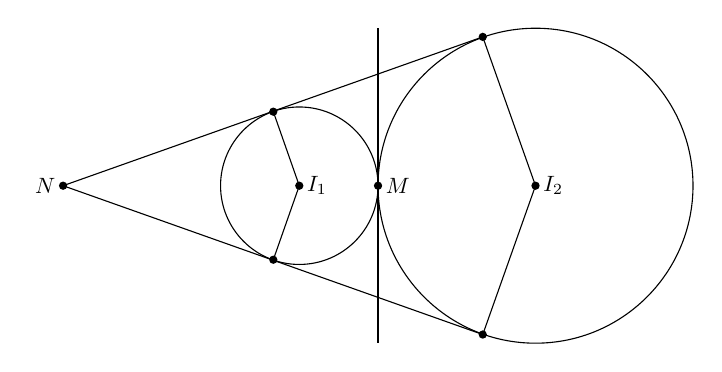
\begin{tikzpicture}
				\draw (1,0) circle (1cm);
				\draw (4,0) circle (2cm);
				\node at (1,0) [right] {$I_1$};
				\fill [fill = black] (1,0) circle (1.5pt);
				\node at (4,0) [right] {$I_2$};
				\fill [fill = black] (4,0) circle (1.5pt);
				\node at (-2,0) [left] {$N$};
				\fill [fill = black] (-2,0) circle (1.5pt);
				\draw (-2,0) -- (3.33, 1.89); \fill [fill = black] (3.33, 1.89) circle (1.5pt);
				\draw (-2,0) -- (3.33, -1.89); \fill [fill = black] (3.33, -1.89) circle (1.5pt);
				\draw (1,0) -- (0.67, 0.94); \fill [fill = black] (0.67, 0.94) circle (1.5pt);
				\draw (1,0) -- (0.67, -0.94); \fill [fill = black] (0.67, -0.94) circle (1.5pt);
				\draw (4,0) -- (3.33, 1.89);
				\draw (4,0) -- (3.33, -1.89);
				\draw (2,2) -- (2,-2);
				\node at (2,0) [right] {$M$}; \fill [fill = black] (2,0) circle (1.5pt);
		\end{tikzpicture}}
		\noindent Gọi $(P)$ là mặt phẳng tiếp xúc cả ba mặt cầu. $(P)$ đi qua $N$ và có véc-tơ pháp tuyến là $\overrightarrow n = (1;a;b)$.
		\begin{align*}
			\Rightarrow{} &\left( P \right) \colon x + 6 + a\left( {y - 2} \right) + b\left( {z - 4} \right) = 0 \\
			\Leftrightarrow{} &\left( P \right) \colon x + ay + bz - 2a - 4b + 6 = 0
		\end{align*}
		\noindent Tiếp tục, ta có
		\begin{align*}
			&\left\{ {\begin{array}{l}
					{d\left( {{I_1};(P)} \right) = 1} \\ 
					{d\left( {{I_2};(P)} \right) = 2} \\ 
					{d\left( {{I_3};(P)} \right) = 3} 
			\end{array}} \right. \\
			\Leftrightarrow{} &\left\{ \begin{array}{l}
				3 = \sqrt {1 + {a^2} + {b^2}} \\
				6 = 2\sqrt {1 + {a^2} + {b^2}} \\
				\left| {4b - 4} \right| = 3\sqrt {1 + {a^2} + {b^2}}  \hfill \\ 
			\end{array}  \right. \\
			\Leftrightarrow{} &\left[ \begin{gathered}
				b = \frac{{13}}{4} \hfill \\
				b =  - \frac{5}{4} \hfill \\ 
			\end{gathered}  \right.
		\end{align*}
		\noindent Với $b = \dfrac{13}{4} \Rightarrow a^2 = -\dfrac{41}{16}$ (loại).
		
		\noindent Với $b = -\dfrac{5}{4} \Rightarrow {a^2} = \dfrac{{103}}{{16}} \Rightarrow a =  \pm \dfrac{{\sqrt {103} }}{4}$.
		
		\noindent Vậy có $2$ mặt phẳng thoả mãn yêu cầu đề bài.
	}
\end{ex}
\Closesolutionfile{ans}
\indapan{6}{ans/ans-C5B3CD3-KQ}